% Options for packages loaded elsewhere
\PassOptionsToPackage{unicode}{hyperref}
\PassOptionsToPackage{hyphens}{url}
\PassOptionsToPackage{dvipsnames,svgnames,x11names}{xcolor}
%
\documentclass[
  authoryear,
  preprint,
  3p]{elsarticle}

\usepackage{amsmath,amssymb}
\usepackage{iftex}
\ifPDFTeX
  \usepackage[T1]{fontenc}
  \usepackage[utf8]{inputenc}
  \usepackage{textcomp} % provide euro and other symbols
\else % if luatex or xetex
  \usepackage{unicode-math}
  \defaultfontfeatures{Scale=MatchLowercase}
  \defaultfontfeatures[\rmfamily]{Ligatures=TeX,Scale=1}
\fi
\usepackage{lmodern}
\ifPDFTeX\else  
    % xetex/luatex font selection
\fi
% Use upquote if available, for straight quotes in verbatim environments
\IfFileExists{upquote.sty}{\usepackage{upquote}}{}
\IfFileExists{microtype.sty}{% use microtype if available
  \usepackage[]{microtype}
  \UseMicrotypeSet[protrusion]{basicmath} % disable protrusion for tt fonts
}{}
\makeatletter
\@ifundefined{KOMAClassName}{% if non-KOMA class
  \IfFileExists{parskip.sty}{%
    \usepackage{parskip}
  }{% else
    \setlength{\parindent}{0pt}
    \setlength{\parskip}{6pt plus 2pt minus 1pt}}
}{% if KOMA class
  \KOMAoptions{parskip=half}}
\makeatother
\usepackage{xcolor}
\setlength{\emergencystretch}{3em} % prevent overfull lines
\setcounter{secnumdepth}{5}
% Make \paragraph and \subparagraph free-standing
\ifx\paragraph\undefined\else
  \let\oldparagraph\paragraph
  \renewcommand{\paragraph}[1]{\oldparagraph{#1}\mbox{}}
\fi
\ifx\subparagraph\undefined\else
  \let\oldsubparagraph\subparagraph
  \renewcommand{\subparagraph}[1]{\oldsubparagraph{#1}\mbox{}}
\fi


\providecommand{\tightlist}{%
  \setlength{\itemsep}{0pt}\setlength{\parskip}{0pt}}\usepackage{longtable,booktabs,array}
\usepackage{calc} % for calculating minipage widths
% Correct order of tables after \paragraph or \subparagraph
\usepackage{etoolbox}
\makeatletter
\patchcmd\longtable{\par}{\if@noskipsec\mbox{}\fi\par}{}{}
\makeatother
% Allow footnotes in longtable head/foot
\IfFileExists{footnotehyper.sty}{\usepackage{footnotehyper}}{\usepackage{footnote}}
\makesavenoteenv{longtable}
\usepackage{graphicx}
\makeatletter
\def\maxwidth{\ifdim\Gin@nat@width>\linewidth\linewidth\else\Gin@nat@width\fi}
\def\maxheight{\ifdim\Gin@nat@height>\textheight\textheight\else\Gin@nat@height\fi}
\makeatother
% Scale images if necessary, so that they will not overflow the page
% margins by default, and it is still possible to overwrite the defaults
% using explicit options in \includegraphics[width, height, ...]{}
\setkeys{Gin}{width=\maxwidth,height=\maxheight,keepaspectratio}
% Set default figure placement to htbp
\makeatletter
\def\fps@figure{htbp}
\makeatother

\usepackage{booktabs}
\usepackage{longtable}
\usepackage{array}
\usepackage{multirow}
\usepackage{wrapfig}
\usepackage{float}
\usepackage{colortbl}
\usepackage{pdflscape}
\usepackage{tabu}
\usepackage{threeparttable}
\usepackage{threeparttablex}
\usepackage[normalem]{ulem}
\usepackage{makecell}
\usepackage{xcolor}
\makeatletter
\@ifpackageloaded{caption}{}{\usepackage{caption}}
\AtBeginDocument{%
\ifdefined\contentsname
  \renewcommand*\contentsname{Table of contents}
\else
  \newcommand\contentsname{Table of contents}
\fi
\ifdefined\listfigurename
  \renewcommand*\listfigurename{List of Figures}
\else
  \newcommand\listfigurename{List of Figures}
\fi
\ifdefined\listtablename
  \renewcommand*\listtablename{List of Tables}
\else
  \newcommand\listtablename{List of Tables}
\fi
\ifdefined\figurename
  \renewcommand*\figurename{Figure}
\else
  \newcommand\figurename{Figure}
\fi
\ifdefined\tablename
  \renewcommand*\tablename{Table}
\else
  \newcommand\tablename{Table}
\fi
}
\@ifpackageloaded{float}{}{\usepackage{float}}
\floatstyle{ruled}
\@ifundefined{c@chapter}{\newfloat{codelisting}{h}{lop}}{\newfloat{codelisting}{h}{lop}[chapter]}
\floatname{codelisting}{Listing}
\newcommand*\listoflistings{\listof{codelisting}{List of Listings}}
\makeatother
\makeatletter
\makeatother
\makeatletter
\@ifpackageloaded{caption}{}{\usepackage{caption}}
\@ifpackageloaded{subcaption}{}{\usepackage{subcaption}}
\makeatother
\journal{Journal Name}
\ifLuaTeX
  \usepackage{selnolig}  % disable illegal ligatures
\fi
\usepackage[]{natbib}
\bibliographystyle{elsarticle-harv}
\usepackage{bookmark}

\IfFileExists{xurl.sty}{\usepackage{xurl}}{} % add URL line breaks if available
\urlstyle{same} % disable monospaced font for URLs
\hypersetup{
  pdftitle={A multi-scale story of the diffusion of a new technology: the web},
  pdfauthor={Emmanouil Tranos},
  pdfkeywords={keyword1, keyword2},
  colorlinks=true,
  linkcolor={blue},
  filecolor={Maroon},
  citecolor={Blue},
  urlcolor={Blue},
  pdfcreator={LaTeX via pandoc}}

\setlength{\parindent}{6pt}
\begin{document}

\begin{frontmatter}
\title{A multi-scale story of the diffusion of a new technology: the
web}
\author[1]{Emmanouil Tranos%
\corref{cor1}%
}
 \ead{e.tranos@bristol.ac.uk} 

\affiliation[1]{organization={University of Bristol and The Alan Turing
Institute},postcode={UK},postcodesep={}}

\cortext[cor1]{Corresponding author}

        
\begin{abstract}
This paper maps the participation in the digital economy and its
evolution in the UK over space and time. Most of the existing economic
geography literature which dealt with the spatiality of the internet
employed supply-side measures, such as infrastructural capacity, in
order to understand the geography of the digital economy and its
potential spatial economic effects. Useful as these approaches might
have been, they cannot capture the micro-processes and the
characteristics of the individual online behaviour. Using large volumes
of archived and geolocated web content, this paper models the diffusion
of web technologies over space and time in the UK. The data and
geolocation strategy allow to capture these processes at a very granular
spatial scale. The modelling approach, which is based on simple spatial
analytical methods and on the estimation of diffusion curves at various
scales, enables to depict the role of geography and other cognitive
factors which drove the diffusion of web technologies. Although the
focus is on a recent historical period -- 1996-2012 -- the results of
the analysis depict diffusion mechanisms which can be very useful in
understanding the evolutionary patterns of the adoption of other newer
technologies.
\end{abstract}





\begin{keyword}
    keyword1 \sep 
    keyword2
\end{keyword}
\end{frontmatter}
    
\section{Introduction}\label{sec-introduction}

Geographers were always interested in how new technologies and
innovations diffuse across space and time and, importantly, how such
spatio-temporal processes can be modeled. After all, diffusion together
with invention and innovation are considered the pillars of
technological change \citep{das2022diffusion}. The seminal contribution
of \citet{hagerstrand1968innovation} is illustrative of this early
interest. However, the torch of exploring and modelling such processes
had been passed to other disciplines such as economics, business studies
and sociology well before the `cultural turn' of economic geography
\citep{perkins2005international}. A potential explanation of the lack of
geographical studies exploring the diffusion of new and, more
specifically for this paper, digital technologies across both space and
time can be attributed to the scarcity of relevant and granular enough
data. As \citet{zook2022mapping} highlight, digital activities are
hardly ever captured in official data.

This paper offers such a contribution: a geographical study illustrating
how a new technology that is the web diffused over space and time in the
UK at a high level of spatial granularity during the \(1996-2012\)
period. It does so by employing a novel source of big data which
captures the active engagement with web technologies during that period.
By addressing this empirical question this paper exemplifies how the
combination of data sources which escape the traditional social science
domain and adequate research methods can offer new lenses to
geographical research regarding the understanding of technological
diffusion.

\textbf{SAY SOMETHING ABOUT SPATIAL ANALYTICS, DIST PAPER BY ARP, NOT
SPECIFIC EXPLANATORY VARIABLES, INTANGIBLE}

The motivation for this paper lies in the fact that there are various
stakeholders who are interested in knowing how new digital technologies
diffused over space and time and use this knowledge to make predictions
regarding the diffusion of related \emph{future} technologies. As per
\citet{leibowicz2016representing}, historical studies agree that
technologies diffuse differently in terms of times, rates, and
geographies and can be driven by related policies \citep{victor1993}.
\citet{meade2021modelling} highlight that a variety of actors have a
direct interest in gaining such knowledge including network equipment
suppliers; network operators, regulatory and local authorities. These
processes and their effects vary a lot across scales: although the
diffusion of a new technology might not be optimal at a local level, it
might be beneficial from a global perspective as it could lead to faster
diffusion to less advantaged places \citep{leibowicz2016representing}.
Despite the spatial heterogeneity of such diffusion mechanisms and the
policy relevance, there are very limited attempts in the literature to
analyse the diffusion of new digital technologies at a detailed
geographical level.

Technological diffusion, which is by definition an aggregated process,
can be discussed in parallel with individual adoption mechanisms. On the
one hand, \citet{rogers2010diffusion} identifies early adopter of new
technologies as `knowledgeable risk takers' and \citet{griliches1957} as
`profit maximisers' \citep{ding2010modeling}. Such individual agents are
rewarded because of their attitude towards new technologies and
innovations. On the other hand, \citet{perkins2011internet} attribute
diffusion to two processes: (i) epidemic-like mechanisms, which are
governed by distance, proximity and social interactions, and (ii)
economic mechanisms as new innovations are adopted by users as they
become more profitable, valueable and useful.

This paper focuses on the diffusion of the web as new technology during
the \(1996-2012\) period. This was an exciting period for digital
technologies as it corresponds with the commercialisation of the
internet and, consequently, its almost universal adoption. The reader is
reminded that it was only in 1994 when Netscape Navigator was
introduced, a year before Microsoft's Internet Explorer.\footnote{\url{https://www.theguardian.com/global/2015/mar/22/web-browser-came-back-haunt-microsoft}}
Also, only \(9\) per cent of UK's households had access to the internet
in \(1998\) \citep{ons2018}, the web included mostly static webpages,
there were no social media and web browsing was happening exclusively
from desktop PCs as there were no smartphones \citep{tranosuk}. Hence,
it is fair to say that the study period captures the very early stages
of the diffusion on a new technology that is the web as well as its
maturity. The former is a key point in the lifecycle of a new
technology. Firstly, during this period new technologies are expensive,
crude and imperfect \citep{rosenberg1994exploring, wilson201281}. A
simple comparison between Web 1.0 and Web 3.0 applications clearly
illustrates this \citep{tranos2020social}; for instance a static website
compared with a platform like \texttt{github}, which enables cooperation
between users and the creation of new information, meaning, and
knowledge \citep{faraj2016special, barassi2012does}. During this period
the performance of a new technology is the main attraction and not the
cost to access and use it \citep{wilson2011lessons}. There is a broader
theoretical discussion in the literature regarding the motivation behind
early adoption. As summarised by \citet{perkins2005international}, on
the one hand, epidemic models highlight the role of interpersonal
contacts as a way for new technologies to diffuse. On the other hand,
economic models underline the importance of heterogeneity. Different
firms have different structures and business plans, which define the
potential economic returns of the adoption of a new technology and,
therefore, the choice to adopt a new technology becomes an individual
option. From a broader and evolutionary perspective, initial conditions
are essential for the creation and evolution of path-dependent
technological development trajectories
\citep{neffke2011regions, simmie2014new}. This argument is even more
relevant when the focus is on digital technologies because of the
commonly found lag between investment and economic returns as reflected
in the Solow paradox
\citep{acemoglu2014return, brynjolfsson2018artificial}.

Importantly, the data used here depicts the \emph{active} engagement
with the web in the UK as it contains all commercial websites that (i)
are part of the UK's relevant second level domain (SLD, .co.uk), (ii)
have been archived by the Internet Archive\footnote{\href{See\%20https://archive.org/}{https://archive.org/}.},
and (iii) include a mention to at least one valid UK postcode in the web
text. The act of creating a website is understood here as active
engagement with the web vis-à-vis the more passive act of browsing the
web or having an internet connection \citep{tranosuk}. Previous studies
have focused mostly on more passive notions of engaging with digital
technologies such as internet adoption and internet speeds
\citep[e.g.][]{blank2018local, riddlesden2014broadband}. More details
about the data and the data generation process can be found in
Section~\ref{sec-datamethods}.

\textbf{S curve??}

\citet{grubler1990rise} Later Hagerstrand conceptualized physical
``barrier'' effects like lakes or uninhabited areas, which, in addition
to distance, act as further retarding effects on diffusion. These are
formalized in the form of ``zero'' or ``half'' contact multiplicators on
the (distance decaying) message flows.

\citet{grubler1990rise} With respect to the formalization of the
communication flows Hagerstrand defines a ``mean information field''
(MIF), in which the probability of communication is a negative function
of distance between individuals

\citet{wilson201281} Logistic growth describes an initial period of
gradual diffusion as a technology is introduced as a new commercial
application, moving then through a rapid, exponential growth phase,
before slowing and eventually saturating \citep{grubler1999dynamics}.
The substitution of incumbent technologies by new competitors leads to
subsequent decline and eventual obsolescence.

\section{Literature review}\label{sec-litreview}

Geographical diffusion is a synthesis of different processes. On the one
hand, a purely spatial or, in other words, contagious processes can be
identified. Adjacency and, more broadly, distance are the key drivers of
diffusion. This perspective draws similarities with epidemics:
innovation just like pathogens spreads because of contagion and,
consequently, proximity and exposure \citep{hivner2003facilitating}. On
the other hand, there is a hierarchical processes. Instead of horizontal
distance-based diffusion mechanisms, the top-down hierarchy of urban
systems shapes technological diffusion. In reality, the synthesis of
these two processes represents how new technologies diffuse over space
and time \citep{morrill2020spatial}.

These ideas were firstly introduced by Torsten Hägerstrand and his
thesis entitled `Innovation Diffusion as a Spatial Process'
\citep{hagerstrand1968innovation}. Hägerstrand was the first one to
identify diffusion as a geographical process. The starting point was the
idea that diffusion is based on passing information through social
networks, which themselves tend to be defined by geography. Hence, he
identified the `neighbourhood' effect of how information, and
consequently, innovation diffuse. He used agricultural innovations to
test and model his ideas using Monte Carlo simulations. Hägerstrand also
incorporated the role of hierarchy and how some phenomena maybe firstly
adopted in larger cities and then diffuse to second tier ones. This is a
sequential instead of a simultaneous process, which resembles the
`lead-lag' spatial acceleration effect in market research
\citep{bento2018time, PERES201091}. Hägerstrand is more widely known
though for highlighting the role time plays in the diffusion of
innovations: an early-pioneering period, a middle fast accelerating
period and a final saturation one \citep{morrill2020spatial}.

The temporal dimension was further explored by Everett Rogers and his
seminal work on `Diffusion of Innovations' \citep{rogers2010diffusion}.
Rogers being a sociologist focused not on the diffusion of innovations
over space and time, but instead on the adoption of new technologies and
innovations by individuals and the individual mechanisms that drive the
decisions behind adoption. He identified five groups of individuals
regarding their adoption speed: innovators, early adopters, early
majority, late majority and laggards. The key mechanism of diffusion and
adoption is communication and how knowledge is transferred within a
social system. Therefore, all approaches agree on the S-shaped diffusion
and cumulative adoption pattern \citep{grubler1990rise}.

Schmidt's Law empirically illustrates a similar pattern. \emph{Core} and
usually highly agglomerated regions is where new technologies are
invented and commercially deployed \citep{grubler1990rise}. This is
where the first adopters tend to be based. Then, technologies spread to
the \emph{rim} and eventually to the \emph{periphery}. Although adoption
pace might be higher when new technologies finally arrive to the
periphery, the saturation levels there may never reach the ones in the
core because of the lack of infrastructure or other necessary
institutions \citep{leibowicz2016representing}. \citet{grubler1990rise}
effectively summarises the three key characteristics of the spatial
diffusion process: (i) the cumulative level of adoption follows an
S-shaped pattern just like purely temporal models; (ii) diffusion is
shaped by a hierarchy effect in a form of a centrifugal force: from core
to periphery; and (iii) diffusion is also shaped by distance and a
neighbourhood effect and contaminate nearby locations. These are the
three mechanisms that the empirical analysis in
Section~\ref{sec-results} investigates.

The remaining of this section reviews empirical studies which analysed
the diffusion on new technologies over space and time. Although the
spatial dimension is present in most of the following studies, the level
of spatial detail is always more coarse than the one adopted here.
\citet{beardsell1999spatial} studied the evolution of the computer
industry in \(317\) US metro areas during the \(1977-1992\) period using
employment data. Their analysis indicated that the relative size
distribution holds for urban computer employment and also urban
heterogeneity is essential in explaining this distribution. In a recent
study, \citet{bednarz2020pulled} focused on wind turbines and modelled
their spatial diffusion across \(402\) German regions during
\(1970-2015\). Their key finding is that local demand than local supply
was the main driving factor.

At a global scale \citet{perkins2005international} explored whther the
diffusion rate of new technologies is driven by a latecomer advantage
and the engagement with the global economy via foreign direct
investments and trade. Their results illustrate that indeed latecomers
and developing countries experience diffusion of new technologies more
rapidly than early adopters and developed countries. At the same scale,
\citet{perkins2011internet} explored whether the adoption of previous
communication technologies that is mail, telegrams and telephones was
shaped by similar socioeconomic factors as the internet. Their results
indicated common patterns regarding the drivers behind the adoption of
different communication technologies.

Turning to studies that share more technological and scalar similarities
with this paper, \citet{ding2010modeling} modelled the spatial diffusion
of mobile telecommunications across regions in China. Their analysis
indicated that socioeconomic characteristics are important determinants
of the timing, speed and the level of mobile diffusion within China.
Using data from a Hungarian online social network,
\citet{lengyel2020role} analysed its adoption and the churn at a very
granular spatial level. Their results are in agreement with early
theoretical and empirical contributions reviewed here: assortativity,
urban scaling and distance are the key drivers of spatial diffusion. At
a global scale \citet{PAPAGIANNIDIS2015308} modelled the diffusion of
different web technologies technologies and practices. Interestingly,
they did so by using similar, but less extensive data as the one used
here. Their analysis illustrated how the diffusion of different web
technologies and practices follow an S-shaped pattern as well as the
different diffusion rates of the different technologies and practices.

All in all, \ldots{}

\section{Data and Methods}\label{sec-datamethods}

\textbf{ADD FAMILY OF WEB TECHNOLOGIES}

To capture the diffusion of web technologies, a website density metric
is developed for two different geographical scales: the Local Authority
Districts (LAD) and the Output Areas (OA). The former is an
administrative unit and there are c.~374 such units in the UK. The
latter is a census-based geographical unit, which is very small as there
are c.~230,000 of them in the UK. This methodological choice will allow
the mapping of the diffusion of web technologies and the assessment of
the diffusion mechanisms at these two very different spatial scales.

The counts of websites at these scales are calculated using data from
the Internet Archive \footnote{\href{See\%20https://archive.org/}{https://archive.org/}.}
and, specifically, the JISC UK Web Domain Dataset \citep{ukwebarchive}.
The Internet Archive is one of the most complete and oldest archive of
webpages in the world operating since 1996
\citep{ainsworth2011much, holzmann2016dawn}. It is a web crawler, which
discovers webpages by following the hyperlinks of every webpage its
archives. This dataset, which is curated by the British Library,
contains all the archived webpages from the UK ccTLD (.uk) from the
1996--2012 period. In essence, this is a long list of 2.5 billion URLs
of archived webpages including also the archival timestamp.

Instead of using the whole .uk country code top-level domain (ccTLD),
this paper focuses on its commercial subset, the .co.uk SLD. This choice
decrease the heterogeneity of the web data as such commercial websites
have rather specific aims: they are used to diffuse information, support
online transactions and share opinions
\citep{THELWALL2000441, blazquez2018big}. Although a UK company can
adopt a generic TLD such as .com and these cases escape the data used
here, such omissions should not affect our results given the popularity
of the .uk ccTLD \citep{tranosuk}: UK consumers prefer to visit a .uk
website when they are searching for products or services \citep{hope};
and anecdotal evidence indicates that during the first half of 2000,
three .co.uk domains were registered every minute \citep{oecd_coms}.
Importantly, previous studies illustrated that .co.uk is the most
popular UK SLD \citep{tranosuk}.

The text from these webpages was scanned using a regular expression
(regex) to identify strings of text which resemble UK postcodes and one
fifth of them included a mention to a postcode \citep{BL2013geo}. This
information allows the geolocation of the data and the creation of the
LAD and OA counts.

The data cleaning process included an aggregation step, through which
the archived webpages were aggregated to the parent websites. This
website reconstruction allows the creation of a \emph{website} instead
of a \emph{webpage} density metric. Websites, which are hierarchical
structures, tend to represent specific orgnanisations or entities, and,
arguably, are more meaningful observational units than webpages, which
ignore the upstream dependencies. Based on the following example, all
three webpages are part of the same website
(\url{http://www.website.co.uk}) and at the end only websites and not
the nested webpages were considered as otherwise the metric would have
been biased towards large, place specific, websites.

\begin{itemize}
\item
  \url{http://www.website.co.uk/webpage_a} B15 2TT
\item
  \url{http://www.website.co.uk/webpage_b} BS8 1TH
\item
  \url{http://www.website.co.uk/webpage_c} B15 2TT
\end{itemize}

\noindent What is challenging is that this aggregation approach, which
has been used elsewhere \citep{tranosuk, shoreditch} may lead to
websites with multiple postcodes. As per the above example,
\href{http://www.website.co.uk}{www.website.co.uk} includes two unique
postcodes: B15 2TT and BS8 1SS. The distribution of postcodes for 2000
is presented in Table \ref{f2000}, which clearly illustrates the wide
range. At the left end of the distribution, there are websites anchored
to a unique location (72\% of all the reconstructed websites in 2000),
which may represent a small company with a single trading location. At
the right end, we have websites with thousands of different postcodes.
Considering the time period of the analysis, such cases can represent
directories which used to be popular in the pre-search engines early
times of the commercial internet \citep{tranosuk}.\footnote{See Figure
  A1 in \textbf{Appendix A in the supplemental data online for
  examples}.}

The analysis presented here is based on two subsets of these data.
Firstly, on websites, which only contain only one unique postcode and,
therefore, the geolocation process does not suffer from noise. As a
robustness check, the analysis is replicated for an extended subset of
websites, which include up to ten unique postcodes. These websites are
geolocated by equally attaching them to multiple locations. This
extended sample includes 94 percent of all the archived websites in
2000.

\begin{table}

\caption{\label{tab:unnamed-chunk-1}Number of unique postcodes per .co.uk website, 2000.\label{f2000}}
\centering
\begin{tabular}[t]{lrrr}
\toprule
Postcodes & F & F (\%) & Cummulative F\\
\midrule
(0,1] & 41,596 & 0.718 & 0.718\\
(1,2] & 6,451 & 0.111 & 0.830\\
(2,10] & 6,163 & 0.106 & 0.936\\
(10,100] & 2,975 & 0.051 & 0.988\\
(100,1000] & 646 & 0.011 & 0.999\\
\addlinespace
(1000,10000] & 62 & 0.001 & 1.000\\
(10000,100000] & 4 & 0.000 & 1.000\\
\bottomrule
\multicolumn{4}{l}{\rule{0pt}{1em}\textit{Source: } Tranos et al. 2021}\\
\end{tabular}
\end{table}

Another data cleaning step dealt with some extreme outliers. Figure
\ref{pc1} plots the website counts for the top 1000 postcodes. Some
obvious outliers can be observed for the 2004-2006 period, which can be
attributed to a link farm \citep{BL2013links}.\\
The website counts for these six postcodes (SE24 9HP, CV8 2ED, GL16 7YA,
CW1 6GL, M28 2SL, DE21 7BF), which in 2004 or 2005 had more than 1000
websites pointing to them, were replaced with predicted values based on
a simple panel regression model with postcode fixed effects and yearly
dummy variables. As the Section~\ref{sec-results} illustrates, this led
to a small increase of the model predictive capability. To put the
magnitude of the data imputation into perspective, this process affected
6 out of the 557,808 postcodes present in the data.

\begin{figure}[H]

{\centering 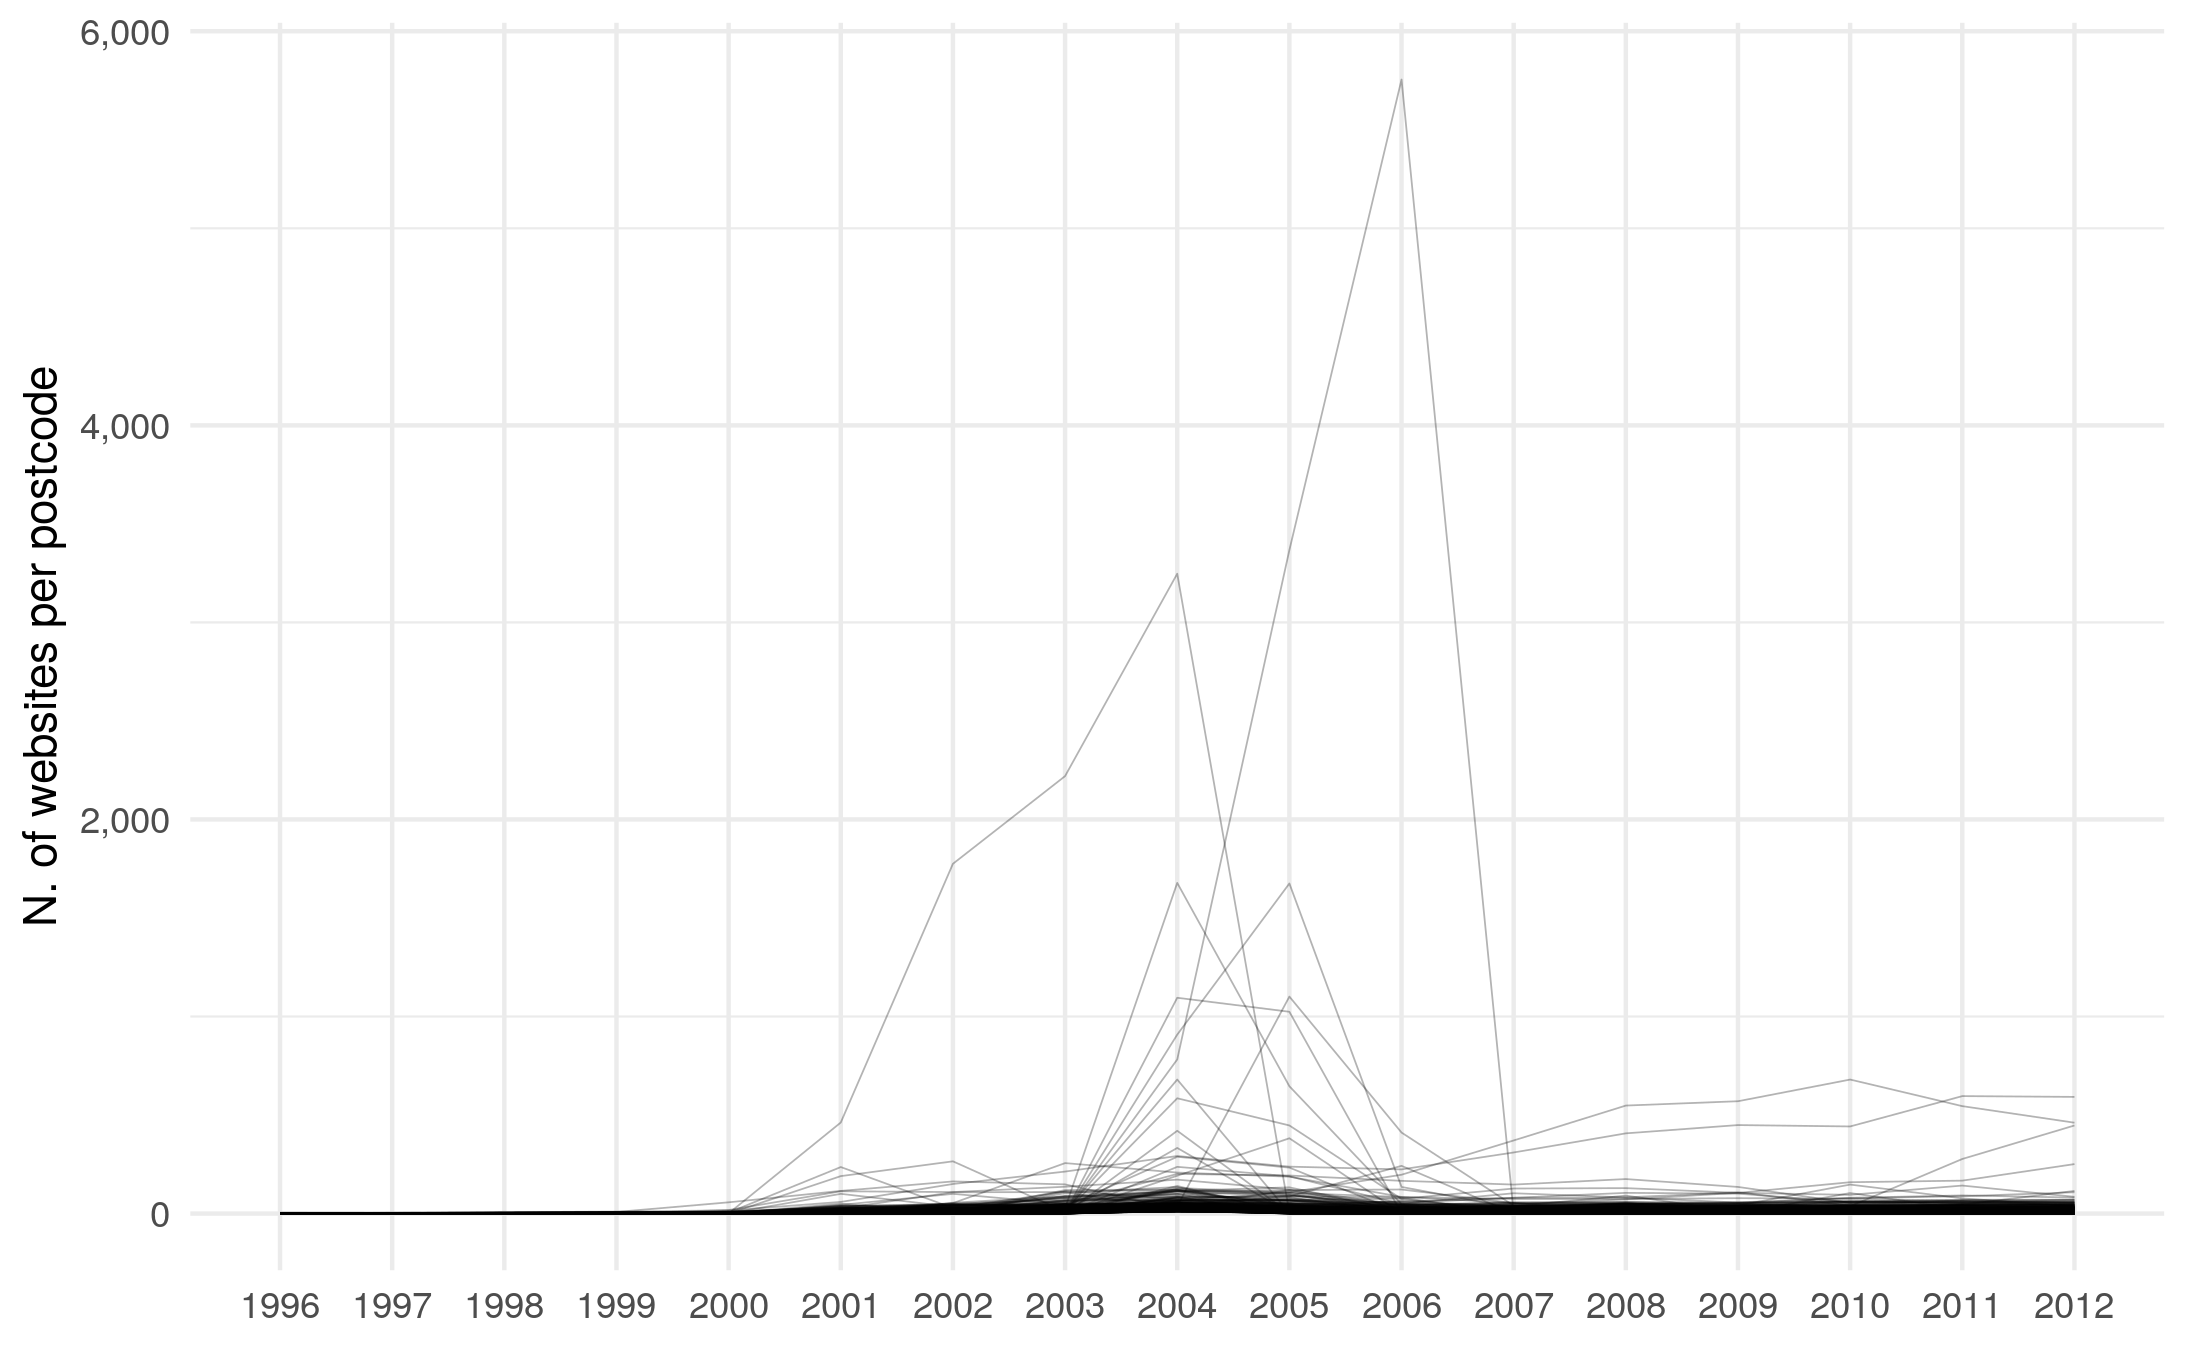
\includegraphics[width=1\textwidth,height=0.6\textheight]{../../outputs/pc_year_1.png}

}

\caption{\label{pc1}Yearly website counts per postcode (top 1000)}

\end{figure}%

To create the website density metric, the yearly website counts at the
LAD level are standardised by the number of firms in LAD to avoid biases
associated with LAD hosting a large number of firms. Given that there is
no such statistic for the OA, the actual OA level counts are used.
However, because of the the consistent spatial definition of OA (they
host 40-250 households),\footnote{\url{https://www.ons.gov.uk/methodology/geography/ukgeographies/statisticalgeographies}}
website counts in OA are interpreted as a density metric too.

These website density metrics are used for the three different steps of
the analysis. Firstly, a system-level analysis explores how the
diffusion of web technologies in the UK fits with the well-established
S-curve. To do so, the following logistic function (Equation \ref{eq:s})
is estimated for the whole of the UK and for each LAD separately:

\begin{align}
y = k /(1 + e^{-(t-t_{o})})\label{eq:s}
\end{align}

\noindent \(k\) is the asymptote or, in other words, the saturation
level, \(b\) the overall growth rate, and \(t_{0}\) the \emph{inflection
point} of maximum growth at \(k/2\), where the logistic function is
symmetrical \citep{wilson201281}. We compare the LAD \(t_0\) of each LAD
against the \(t_0\) of the UK to delineate whether a LAD reached that
point faster or slower than the country average. Importantly, an
accuracy criterion was imposed and only S-curves with \(R^2 > 0.9\) were
included in the analysis. To estimate Equation \ref{eq:s} a
self-starting logistic growth model was employed using the \texttt{nls}
and \texttt{SSlogis} functions in \texttt{R}.

The system-level analysis also focuses on the volatility of the web
adoption to depict places with high concentration of early adopters and,
equally, latecomers. To do so, the change of the ranking of the UK LAD
over time is plotted and discussed. Both the S-curve and the volatility
analysis focus only on LAD as the very large number of OA would have
made such analysis diffucult to visualise and interpret.

Next, exploratory spatial data analysis depicts whether the two main
drivers of spatial diffusion -- namely neighbourhood and hierarchy --
underpin the diffusion of web technologies in the UK. To capture the
former and following \citet{ding2010modeling} the Moran's I and the
Local Index of Spatial Association (LISA) are estimated for website
density. To address the hierarchy mechanism, the Gini coefficient -- a
well established metric of inequality -- is calculated. All the above
are computed and plotted longitudinally both for the LAD and the OA.

Lastly, a modelling framework is developed to test the above diffusion
mechanisms. The overarching aim is to build a model that can test the
relationship between the website density and these mechanisms:

\begin{align}
Website\,Density_{t} \sim Hierarchy_{t-1} + Neighbourhood_{t-1} + S-curve_{t}\label{eq:rf.generic}
\end{align}

To estimate Equation \ref{eq:rf.generic}, Random Forest (RF) models were
built. This is a popular machine learning algorith for both regression
and classification problems \citep{biau2012analysis}. It was introduced
by \citet{breiman2001random} and has\\
gained popularity, becoming a go-to data science tool. RF can
effectively handle skewed distributions and outliers, model non-linear
relationships, require minimal hyperparameter tuning, exhibit low
sensitivity to these parameters, and have relatively short training
times \citep{Caruana2008, liaw2002classification, yan2020using}. These
attributes match well with the website density data characteristics
including skewness especially for OA. Also, the large data size (c.~230k
data points for each of the 17 years) call for fast training times.
Importantly, RF predictions tend to be more accurate than those from
single regression trees and outperform Ordinary Least Squares in
out-of-sample predictions, even with moderate-sized training data and a
small number of predictors
\citep{mullainathan2017machine, athey2019machine, sulaiman2011intelligent, pourebrahim2019trip, biau2012analysis}.

RF is a tree-based ensemble learning algorithm
\citep{breiman2001random}. It begins by generating random samples of the
training data, which are then used to grow regression trees to predict
the dependent variable. Data points and predictors are randomly sampled
for the different trees. The trees are trained in parallel using their
own bootstrapped samples of the training data. A crucial feature of RF
is their ability not to overfit, meaning they can generalize well to
unseen test data. While each tree may overfit individually, the ensemble
of trees does not because the errors of individual trees are averaged,
reducing the overall variance and preventing overfitting
\citep{last2002improving}. For regression problems, RF predictions are
made by averaging the predictions of all decision trees.

RF have been widely employed to address regression research problems.
\citet{pourebrahim2019trip} combined a spatial interaction modeling
framework with ML algorithms including RF to predict commuting flows in
New York City. \citet{sinha2019assessing} advocated for adopting spatial
ensemble learning approaches, such as RF, to model spatial data with
high autocorrelation and heterogeneity. \citet{creditspatial} predicted
employment density in Los Angeles using spatially explicit RF.
\citet{guns2014recommending} used RF to build a recommendation system
for research collaborations. \citet{ren2019predicting} trained RF to
predict the socio-economic status of cities using various online and
mobility predictors. \citet{tranos2023using} utilised hyperlinks data
and RF to make out-of-sample predictions of interregional trade.
\citet{zhou2023geography} employed such a framework to assess whether
key predictors of obesity differ across English cities.

\section{Results}\label{sec-results}

\begin{enumerate}
\def\labelenumi{\arabic{enumi}.}
\item
  S-shaped diffusion curves: S for LAD per firm. UK, fast/slow/examples
\item
  ranks: there is stability and movement
\item
  Neighbourhood effect: diffusion proceeds outwards from innovation
  centers, first ``hitting'' nearby rather than far-away locations
  (Grubler 1990)
\end{enumerate}

\begin{itemize}
\item
  Moran's I: for OA and LAD over time
\item
  LISA maps: for OA and LAD over time More and less expected clusters.
  Different scales show different results
\end{itemize}

\begin{enumerate}
\def\labelenumi{\arabic{enumi}.}
\setcounter{enumi}{3}
\tightlist
\item
  Hierarchy effect: from main centers to secondary ones -- central
  places
\end{enumerate}

\begin{itemize}
\tightlist
\item
  Gini coefficient. Almost perfect polarisation of web adoption in the
  early stages at a granular level More equally diffused at the Local
  Authority level Plateau overtime
\end{itemize}

\begin{enumerate}
\def\labelenumi{\arabic{enumi}.}
\setcounter{enumi}{4}
\tightlist
\item
  RF
\end{enumerate}

\begin{itemize}
\tightlist
\item
  ideal: (i) train RF for all years and all (1) LAD and (2) OA with CAST
  and report metrics. (ii) train for all years and all but one region
  for (1) LAD and (2) OA to predict to the holdout region. Reports
  predictions as region similarities.
\end{itemize}

Figure \ref{s_uk} plots the S curve for the cumulative adoption of
website technologies in the UK during the 1996-2012 period. It
demonstrates a pattern well aligned with previous studies discussed in
Section~\ref{sec-litreview}. The vertical line for year 2003 illustrates
the point where the modeled cumulative adoption was equal to 50\% of the
maximum. This \(t_0\) \emph{inflection} point signals the maximum
adoption speed and is used here to determine whether the UK LAD reached
that inflection point earlier or later than the UK average.
Specifically, the S curve and the inflection point are estimated for
every LAD individually and then compared with the UK average. LAD that
reached their inflection point earlier than the country average are
labelled as \emph{fast} and the rest as \emph{slow}. Figure \ref{s_map}
maps this pattern and the picture is not entirely clear. On the one
hand, there are some expected examples of LAD with relevant industrial
backgrounds delineated as fast: the City of London, a world-renowned
cluster of finance industries \citep{cook2007role}, and Reading, a town
with high-tech service industries in proximity to London and its main
airport, Heathrow \citep{england2005polynet}. On the other hand, LAD
which were expected to appear as fast -- e.g.~Hackney in central London
and Bristol, a well-established creative cluster
\citep{oatley1999cultural, bassett2002cultural} -- were delineated as
slow. Nevertheless, out of the 10 fastest LAD, eight were located in
Greater London and one in Cambridge (see \textbf{Appendix}), but in
overall there is a spatially heterogenous and not easy to explain
spatial pattern.

\begin{figure}[H]

{\centering 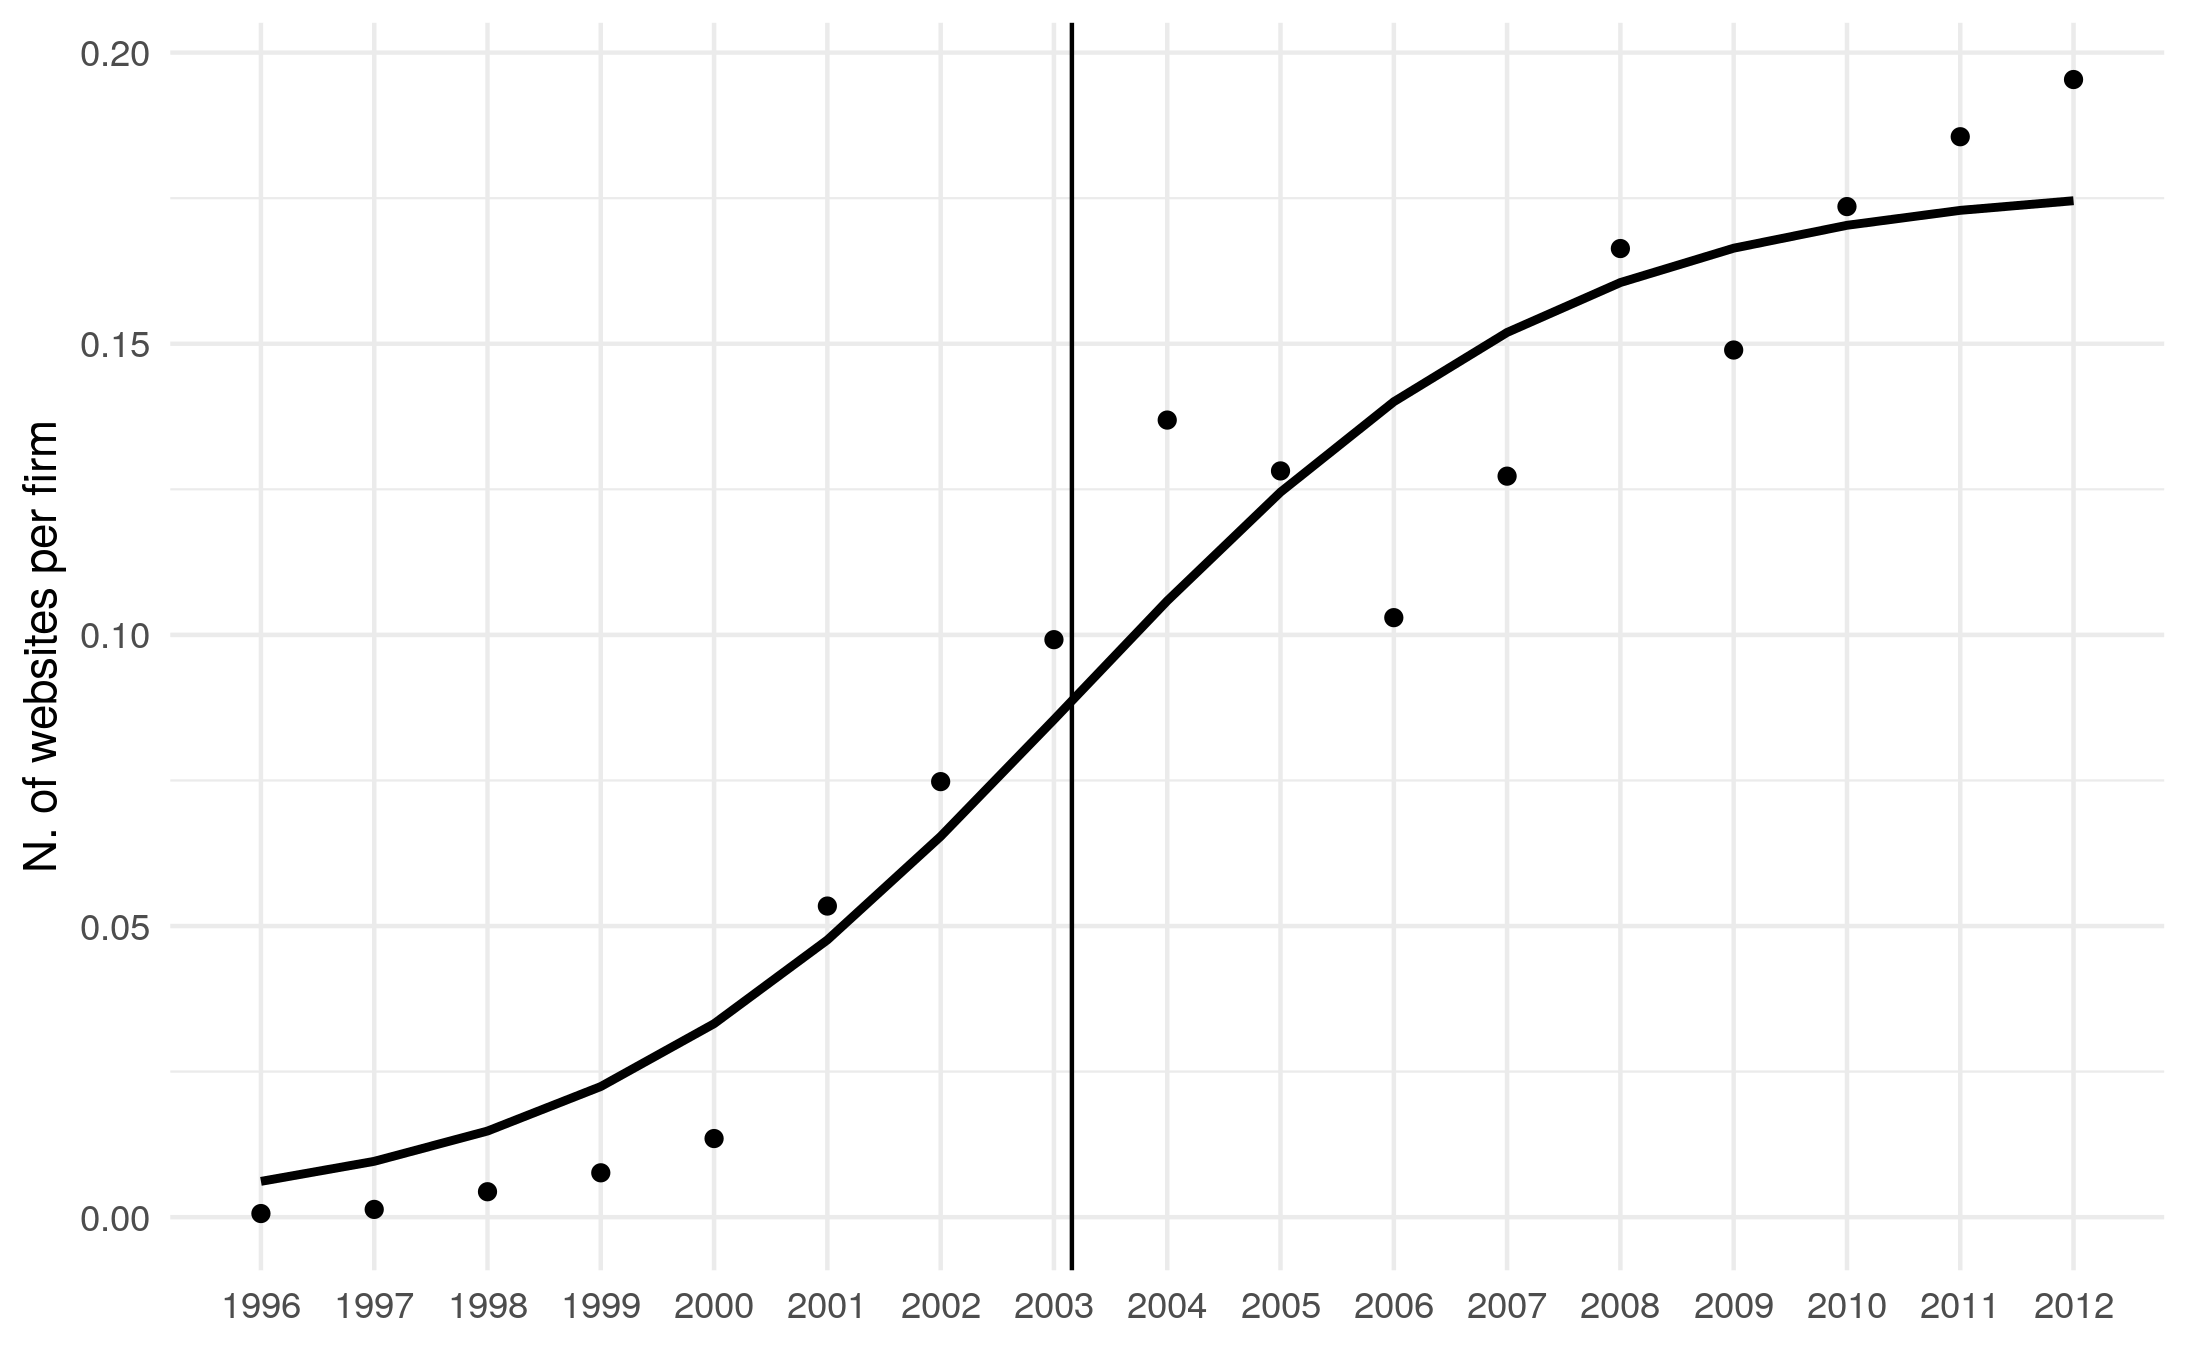
\includegraphics[width=1\textwidth,height=\textheight]{../../outputs/s/s_uk_per_firm.png}

}

\caption{\label{s_uk}Grwoth curve, UK}

\end{figure}%

\begin{figure}[H]

{\centering 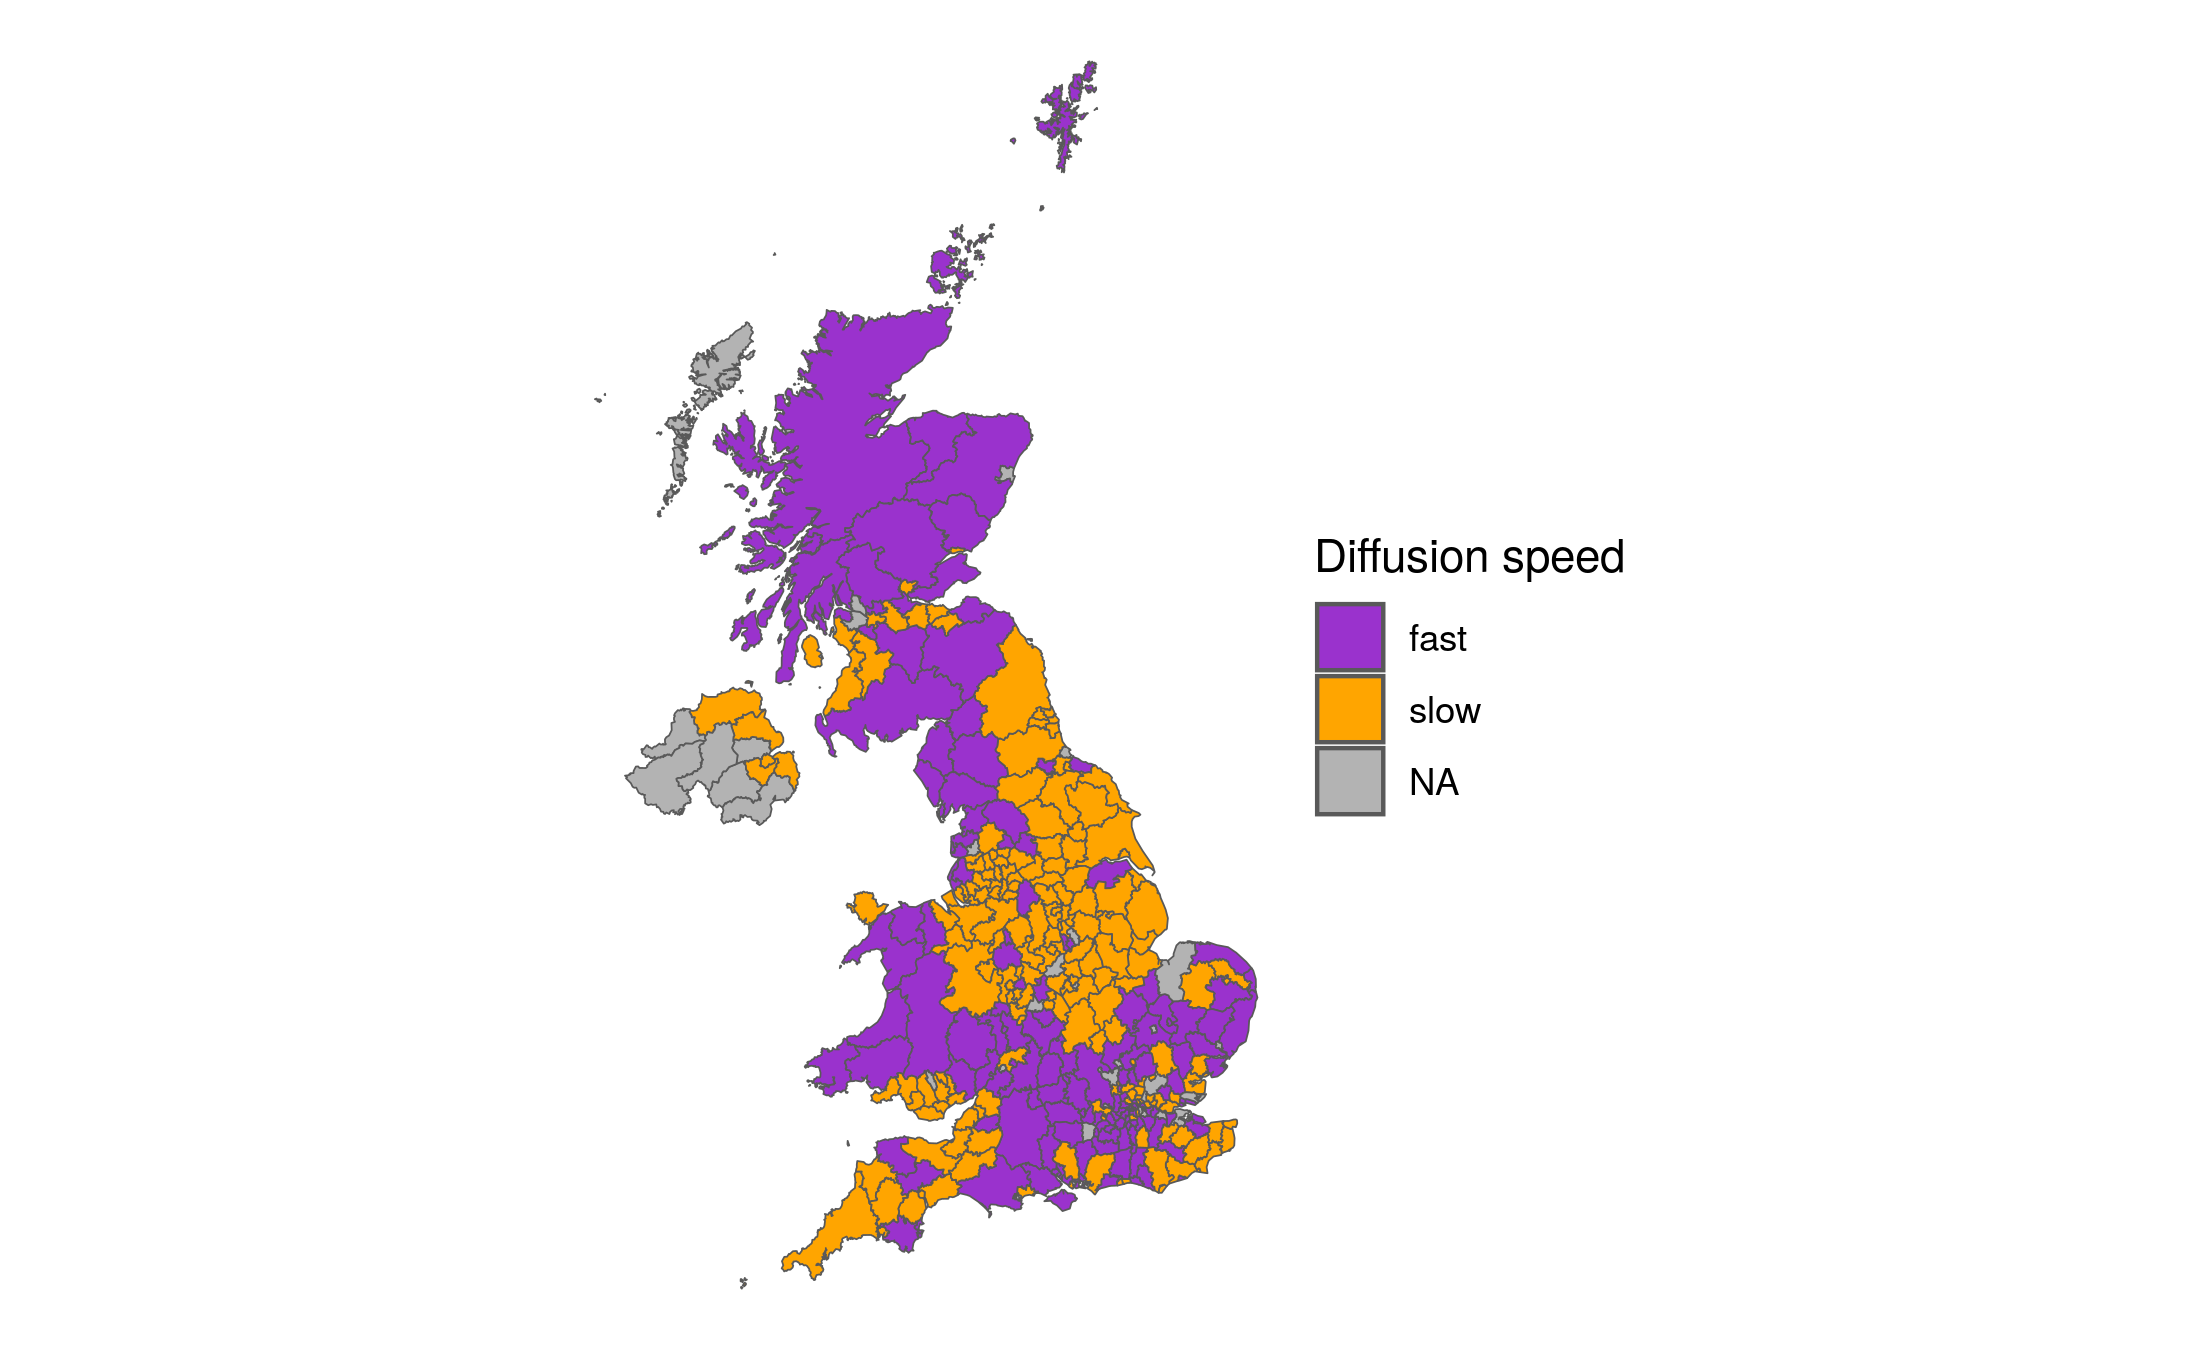
\includegraphics[width=1\textwidth,height=\textheight]{../../outputs/s/speed_map.png}

}

\caption{\label{s_map}LAD adoption rates}

\end{figure}%

The next step is to assess the stability and volatility of the LAD in
terms of their adoption of web technologies. As we know from the
literature \citep{risk_perceptions}, different agents have different
perceptions about and levels of acceptance of the risks and the
potential economic returns associated with the adoption of new
technologies -- see for instance the seminal work of
\citet{venkatesh2000theoretical}. To reveal such aggregated patterns,
Figures \ref{rank_stable} and \ref{rank_unstable} plot the ranking of UK
LAD based on website density. To decrease noise, the average ranking of
1996-1998 and 2010-2012 is plotted instead of the individual years.
While there are quite a few obvious cases of LAD that maintained their
position between the beginning and the end of the study period either at
the top or at the bottom of the hierarchy (Figure \ref{rank_stable}),
there are also quite a few LAD that changed drastically their position.
Some of these LAD enjoyed a process that at the first instance looks
like leapfrogging since they managed to jump at the top of the hierarchy
despite their slow start (top of Figure \ref{unstable}). There is
extensive literature regarding the potential benefits of technological
leapfrogging. The underpinning argument is that latecomers can adopt and
benefit from new technologies that have been developed elsewhere without
incurring the hefty initial R\&D costs \citep{teece2008firm}. Although
the leapfrogging literature does not pay much attention to cities and
regions \citep{yu2018sustainability}, previous research highlighted the
long term and sustained productivity benefit of the early adopters of
web technologies in the UK \citep{tranosuk}. So, although the LAD system
is volatile, it is not clear whether the LAD with high concentration of
late adopters will gain any latecomer benefits in a way similar to
countries experiencing such technological leapfrogging.

\begin{figure}[H]

{\centering 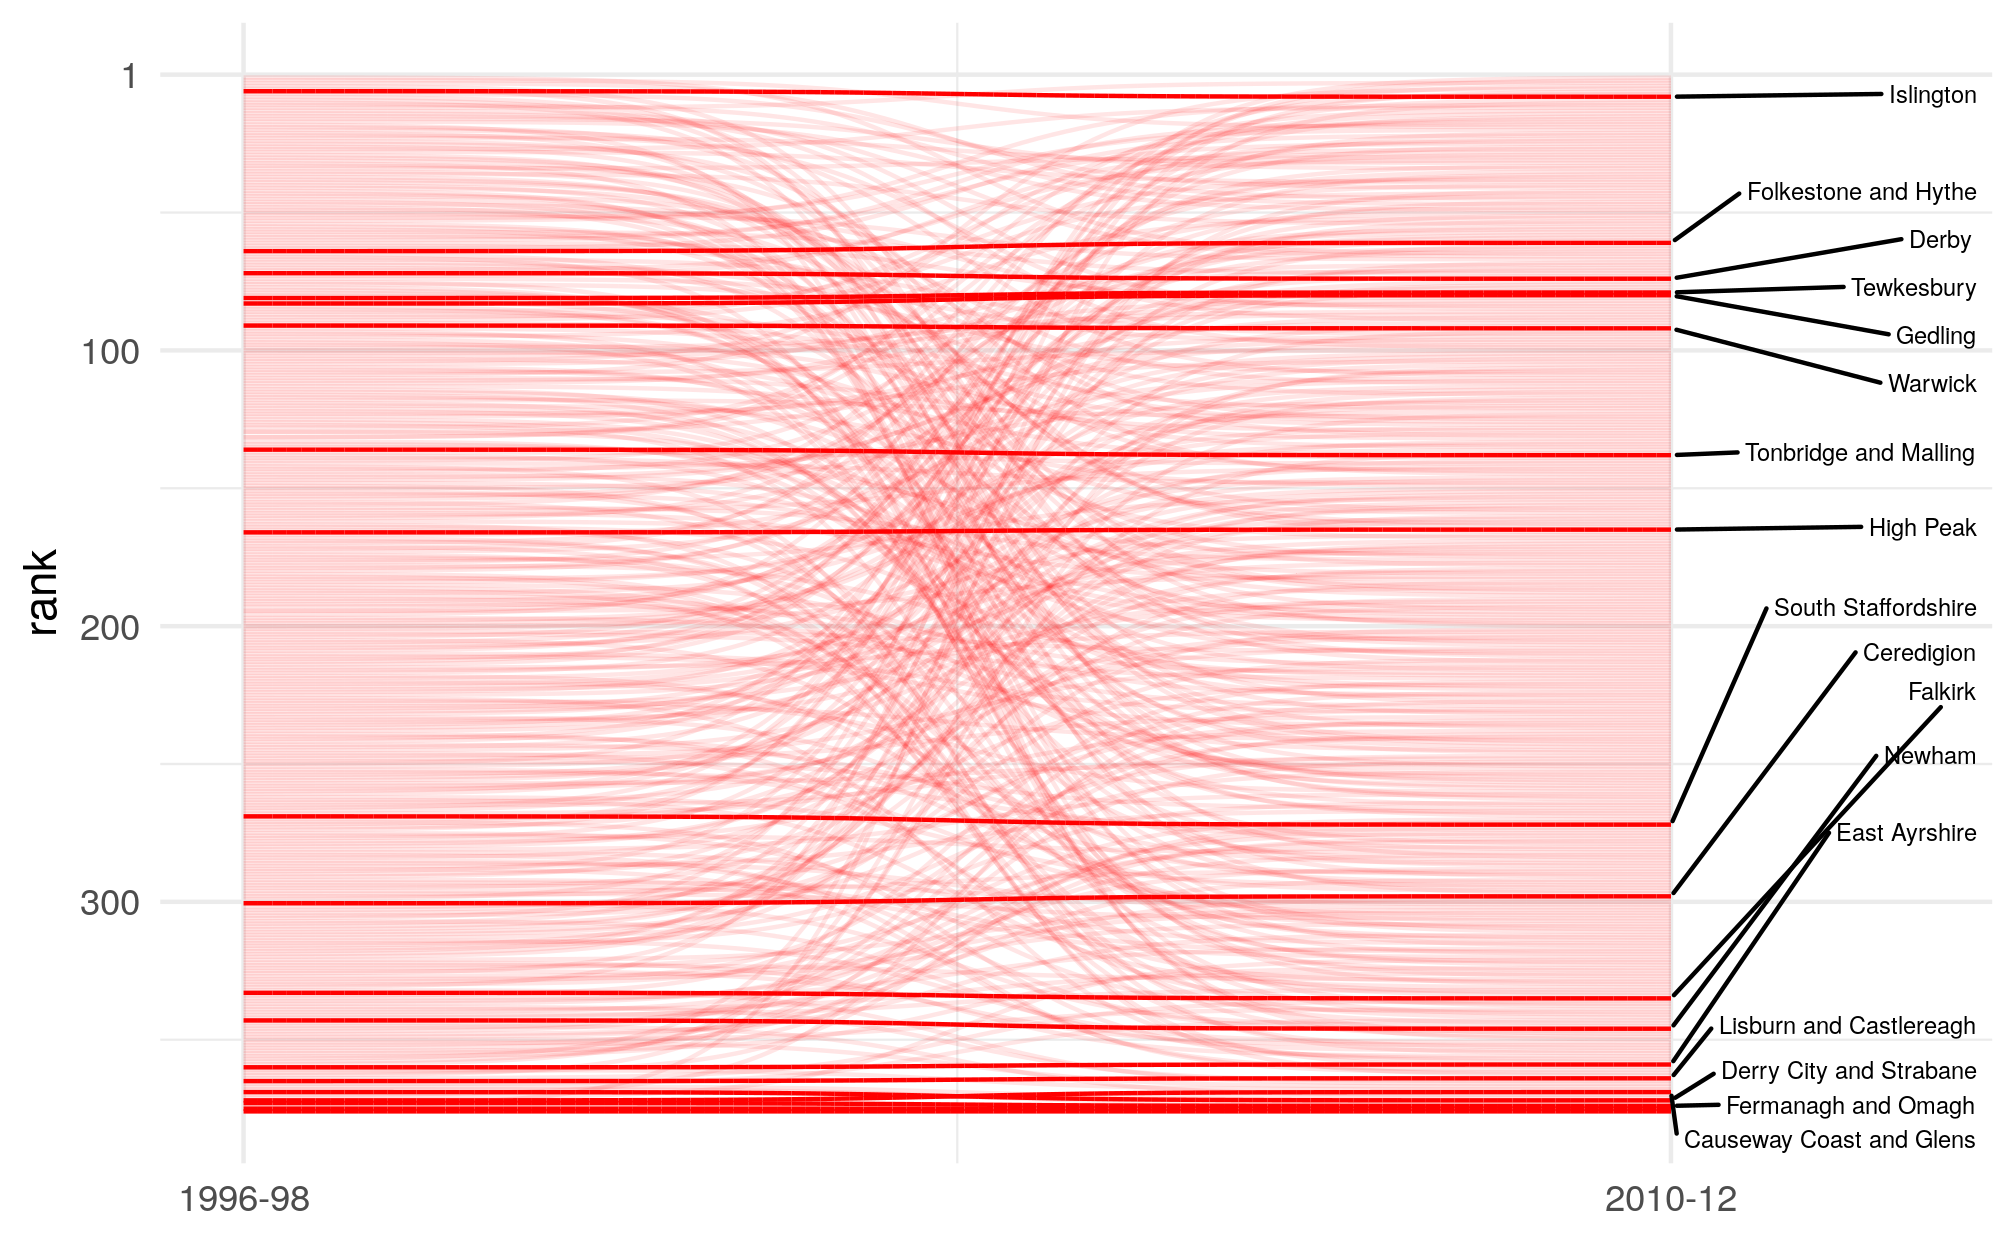
\includegraphics[width=1\textwidth,height=\textheight]{../../outputs/ranks/web_per_firm2000_2012_only05_av.png}

}

\caption{\label{rank_stable}Dynamics of wed diffusion: stability of LAD}

\end{figure}%

\begin{figure}[H]

{\centering 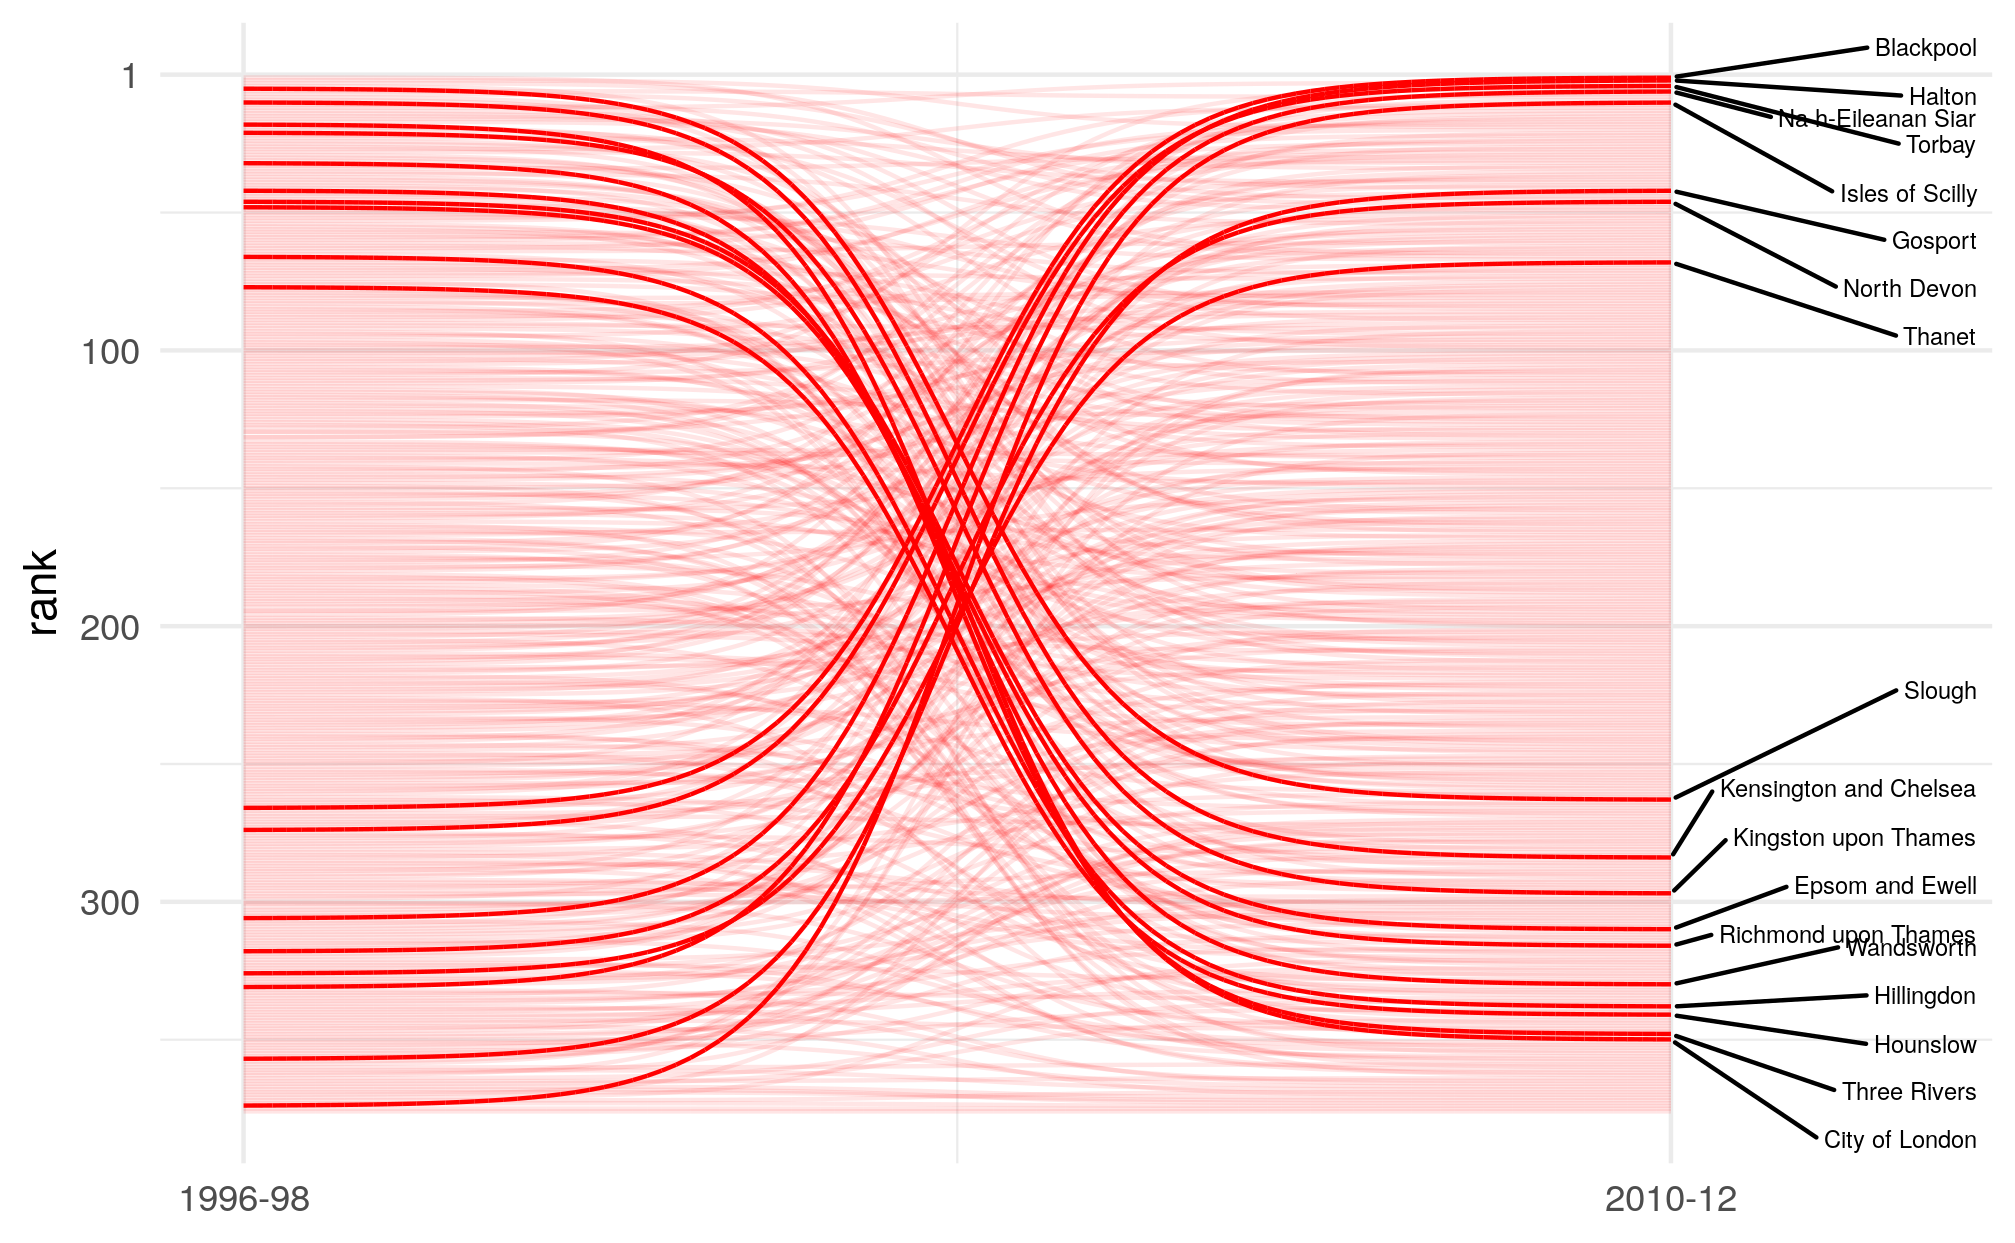
\includegraphics[width=1\textwidth,height=\textheight]{../../outputs/ranks/web_per_firm2000_2012_only95_av.png}

}

\caption{\label{rank_unstable}Dynamics of wed diffusion: volatility LAD}

\end{figure}%

Then, figures \ref{morani} and \ref{lisa} offer a first insight into
whether a neighbourhood effect underpins the diffusion of web
technologies in the UK as they plot the Moran's I and the LISA maps of
website density respectively for LAD and OA. Starting from the former,
spatial autocorrelation was higher in the beginning and then around year
2000 dropped slightly and stabled at 0.2. This reflects the early
concentration of high website density around London, which over time
diffused as high-high clusters can be seen in other parts of the country
away from London as seen in Figure \ref{lisa}. An almost reverse pattern
can be observed for OA. At the beginning of the study period Moran's I
was around 0.1 and it plateaued after 2000-2001 around 0.2. Because of
the very small size of OA, at the early stages of the diffusion of web
technologies their adoption was spatially scattered. This is reflected
in the lack of any significant clusters in 1996. Eventually, as the
adoption rate increased, more such clusters of high website density were
formed and this is reflected both in the Moran's I and the LISA maps in
Figures \ref{morani} and \ref{lisa}. All in all, the exploratory spatial
data analysis advocates towards an underpinning neighbourhood effect and
the different scales of analysis illustrate how it evolved differently
over time.

\begin{figure}[H]

{\centering 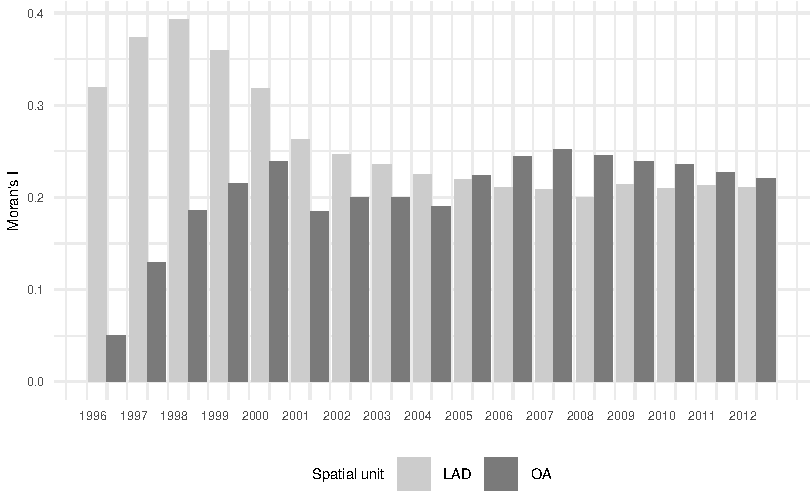
\includegraphics[width=1\textwidth,height=\textheight]{tranos2023_files/figure-pdf/morani-1.pdf}

}

\caption{\label{morani}Website density Moran's I}

\end{figure}%

Figure \ref{lisa}

\begin{figure}[H]

{\centering 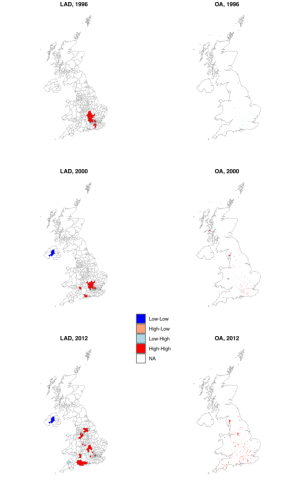
\includegraphics[width=1\textwidth,height=0.8\textheight]{tranos2023_files/figure-pdf/unnamed-chunk-7-1.pdf}

}

\caption{\label{lisa}\centering Website density LISA maps}

\end{figure}%

To illustrate whether a hierarchical process underpins the diffusion of
web technologies, the Gini coefficient is calculated yearly both for LAD
and OA. As a metric of inequality, the Gini coefficient demonstrates
whether website density is concentrated in a small number of LAD/OA, or
whether it is more equally spread across the country. Both scales of
analysis in Figure \ref{gini} illustrate the same picture. At the
beginning of the commercial internet website density was extremely
unequal, or in other words, only a few places had websites associated
with them. Inequality dropped and plateaued after 2000 for both scales
illustrating that at the first stages of the commercial internet,
website density was concentrated in a limited number of places. This is
an indication of a hierarchical diffusion mechanism that led over time
to a more equal spread. Interestingly, the year 2000 is again a period
of change for this diffusion mechanisms as it was for the neighbourhood
process. There is a substantial difference between the Gini coefficient
magnitude for LAD and OA, but this is well expected as the very small
size of OA equates to a lot polygons without any websites pointing to
them -- for instance residential OA. LAD/OA

\begin{figure}[H]

{\centering 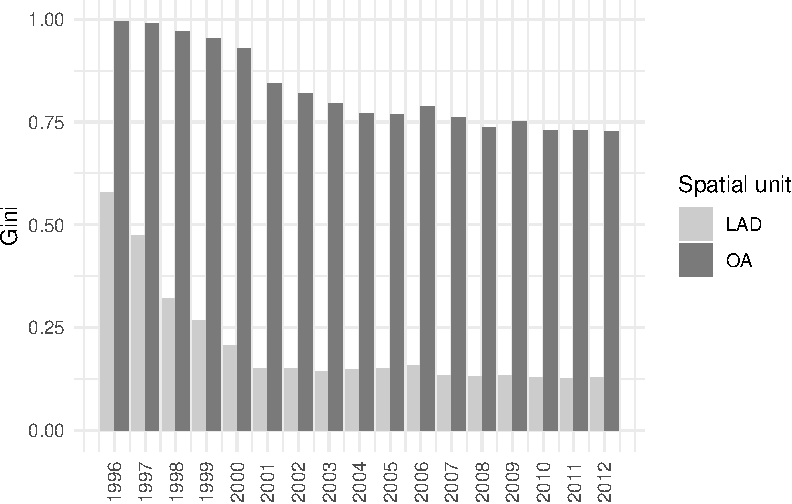
\includegraphics[width=1\textwidth,height=\textheight]{tranos2023_files/figure-pdf/gini-1.pdf}

}

\caption{\label{gini}Website density Gini coefficient}

\end{figure}%

The next section incorporates the above discussed spatial processes of
the diffusion of web technologies into a modelling framework. The aim is
to use variables depicting these spatial processes in order to predict
the diffusion of web technologies in the UK over space and time and
across different scales. Specifically, four different models are
estimated. Firstly, all the data points for the OA and LAD are utilised
in order to build two respective RF models and assess their capacity to
predict the adoption of web technologies. These two models will reveal
the predictive capacity of the diffusion mechanisms and also allow to
see how the importance of such variables changes across scales. The next
two sets of models will be again trained on web diffusion at the two
working scales: OA and LAD. However, instead of using all the data
points, the OA and the LAD from one of the twelve UK regions are held
out and then the trained model is used to predict website density in the
OA or the LAD of the held-out region. This process takes place
recursively for all UK regions. The difference in the predictive
capacity of the different samples will reveal how dissimilar are these
spatial process across regions and, importantly, at different scales.

It needs to be highlighted here that the cross-validation for all models
is spatially and temporally sensitive. Instead of using 10 random folds,
we employ the \texttt{CAST} package which allows holding back data
points from specific years and spatial units and use them for testing in
order to estimate the model performance \citep{meyer2018improving}.

The models include variables that capture the three processes that the
relevant literature and the descriptive analysis presented above
highlighted. Namely, the models capture: (i) a hierarchy effect with
diffusion running from main centres to secondary ones, (ii) a
neighborhood effect according to which diffusion first hits nearby
locations, and (iii) the rather canonical pattern of diffusion over time
as reflected in the S-shaped pattern in the cumulative level of
adoption.

To capture the hierarchy effect the models include as predictors a one
year lag of website density in London, the largest city in the UK, a one
year lag of the website density in the nearest city and the same for the
nearest retail centre. Due to the small sizes of the retail centres, the
latter is only relevant for the OA-level models. In addition, the models
include the distance to London, the nearest city and the nearest retail
centre. The underlying logic is that the level of website adoption in a
spatial unit depends on the level of the adoption in places further up
in the urban hierarchy the previous year. The inclusion of the distance
variables incorporates spatial structure into the hierarchy argument. To
depict the neighbourhood effect, the website density of the neighbouring
spatial units in the previous year is employed. Again, the underpinning
rationale is that the level of web adoption within a spatial unit
depends on the level of web adoption in the neighbouring spatial units
the year before. This represents the `hitting nearby locations first'
argument. Therefore, the spatial and temporal lag of the website density
in LAD and OA is calculated. Lastly, the time effect which is reflected
on the S-curve for the cumulative adoption is captured by a time trend
variable. Hence, all four model will follow the following generic form
(Eq. \ref{model}):

\begin{align} \label{model}
Website\,Density_{t} \sim Distance\,London +
Website\,density\,London_{t-1} +\notag\\
Distance\,Nearest\,City +
Website\,density\,Nearest\,City_{t-1} +\notag\\
Distance\,Nearest\,Retail_{i} +
Website\,density\,Nearest\,Retail_{t-1} +\notag\\
W*\, Website\,density_{t-1} +\notag\\ 
year_{t}
\end{align}

To assess the predictive capability of the model, three broadly utilised
metrics are employed: the coefficient of determination (\(R^2\)), mean
absolute error (MAE) and root mean square error (RMSE):

\begin{align}
R^2 = 1 - \frac{\sum_{k} (y_{k} - \hat{y_{k}})^2} {\sum_{k} (y_{k} - \overline{y_{k}})^2} \label{eq:rsquared}
\end{align}

\begin{align}
MAE = \frac{1}{N} \sum_{k = 1}^{N} |\hat{y_{k}} - y_{k}| \label{eq:mae}
\end{align}

\begin{align}
RMSE =  \sqrt{\frac{\sum_{k = 1}^{N} (\hat{y_{k}} - y_{k})^2} {N}} \label{eq:rmse}
\end{align}

\(y_{k}\) is the \(k^{th}\) observation of the dataset, which consists
of \(N\) observations in total. \(\hat{y_{k}}\) is the \(k_{th}\)
predicted value for the dependent variable and \(\overline{y_{k}}\) is
the average value of \(y\). The last two metrics are expressed in the
same units as the dependent variable -- websites per firm for the LAD
modes and the number of websites for the OA models -- while the first
one is the coefficient of determination between the observed and the
predicted values of website adoption. Regarding \(MAE\), it is the
absolute difference between the observed and the predicted website
adoption. While \(MAE\) does not penalise for large errors, \(RSME\)
does so as it is proportional to the squared difference between the
observed and the predicted trade flows. Hence larger errors weigh more
for \(RMSE\) \citep{pontius2008components}.

Table~\ref{tbl-model-metrics} presents the model performance for the
first set of models, for which all data points are employed for training
and testing via cross validation. The first one is trained and tested on
374 LAD and the second on 232,296 OA, both for a 16 year period
(1997-2012). The results are remarkably good considering that the are
the outcome of space and time sensitive CV, so the the model does not
suffer from overfitting. At the LAD level the model predicts 81\% of the
variation of website density. Both error metrics indicate that the model
error is \((\frac{1}{20}, \frac{1}{30})\) of a website per firm. At the
OA the \(R^2\) drops down to 21\%. Considering its granularity, this is
still a remarkable performance. To contextualise it, the model results
in a MAE of one website for areas small enough to host less than 140
households.\footnote{According to the Office for National Statistics,
  80\% of OA in England and Wales host 110-139 households,
  \href{https://www.ons.gov.uk/census/2001censusandearlier/dataandproducts/outputgeography/outputareas}{www.ons.gov.uk}.}
Because of the small size of the spatial units, the distribution is
highly skewed and a significant part of them is not linked to any
websites. In 1997 only 1\% of the UK OA were associated with at least
one website. This should not come as a surprise as this was the very
beginning of the commercial internet and any activities with a digital
footprint were concentrated in a handful of areas. This was clearly
illustrated in Figure \ref{lisa}. At the end of the study period almost
half of the UK OA were not associated with a website. Again, given the
granularity of the data this should not come as a surprise.

\begin{longtable}[]{@{}llll@{}}
\caption{Model metrics}\label{tbl-model-metrics}\tabularnewline
\toprule\noalign{}
& RMSE & \(R^{2}\) & MAE \\
\midrule\noalign{}
\endfirsthead
\toprule\noalign{}
& RMSE & \(R^{2}\) & MAE \\
\midrule\noalign{}
\endhead
\bottomrule\noalign{}
\endlastfoot
Local Authorities & 0.032 & 0.810 & 0.019 \\
Output Areas & 5.000 & 0.205 & 1.047 \\
\end{longtable}

Figures \ref{var.imp.LAD} and \ref{var.imp.OA} plot the importance of
the different predictors. When the focus is on the LAD, the website
density in the nearest city, in London and in the neighbouring LAD the
year before are the most important predictors. They are followed by the
yearly trend, while the spatial configuration as reflected in distances
to London or the nearest city only play a minor role. This can be
attributed to the rather coarse spatial scale of analysis. Nevertheless,
all previously discussed spatial processes are at play in the diffusion
of web technologies at the LAD level: the first two predictors depict
the hierarchical effect, the spatial and temporal lag of website density
depict the neighbourhood effect and the yearly trend the time-sensitive
cumulative adoption pattern.

When the much more granular scale of OA is adopted, the picture is
reversed. The most important predictors are the three distance variables
to London, the nearest city and the nearest retail centre. They stil
depict the hierarchical effect, but proximity to the different
population centres is more important than their lagged web densities in
predicting website diffusion. The neighbouring effect is less important
at this scale. What is interesting is the almost negligible role of the
yearly trend and London's website density. While the former probably
illustrates the large heterogeneity in how web technologies have been
adopted at this very fine scale, the later highlights that the
importance of past web adoption rates in large population centres is
surpassed by proximity to them and spatial configuration at this scale.

\begin{figure}[H]

{\centering 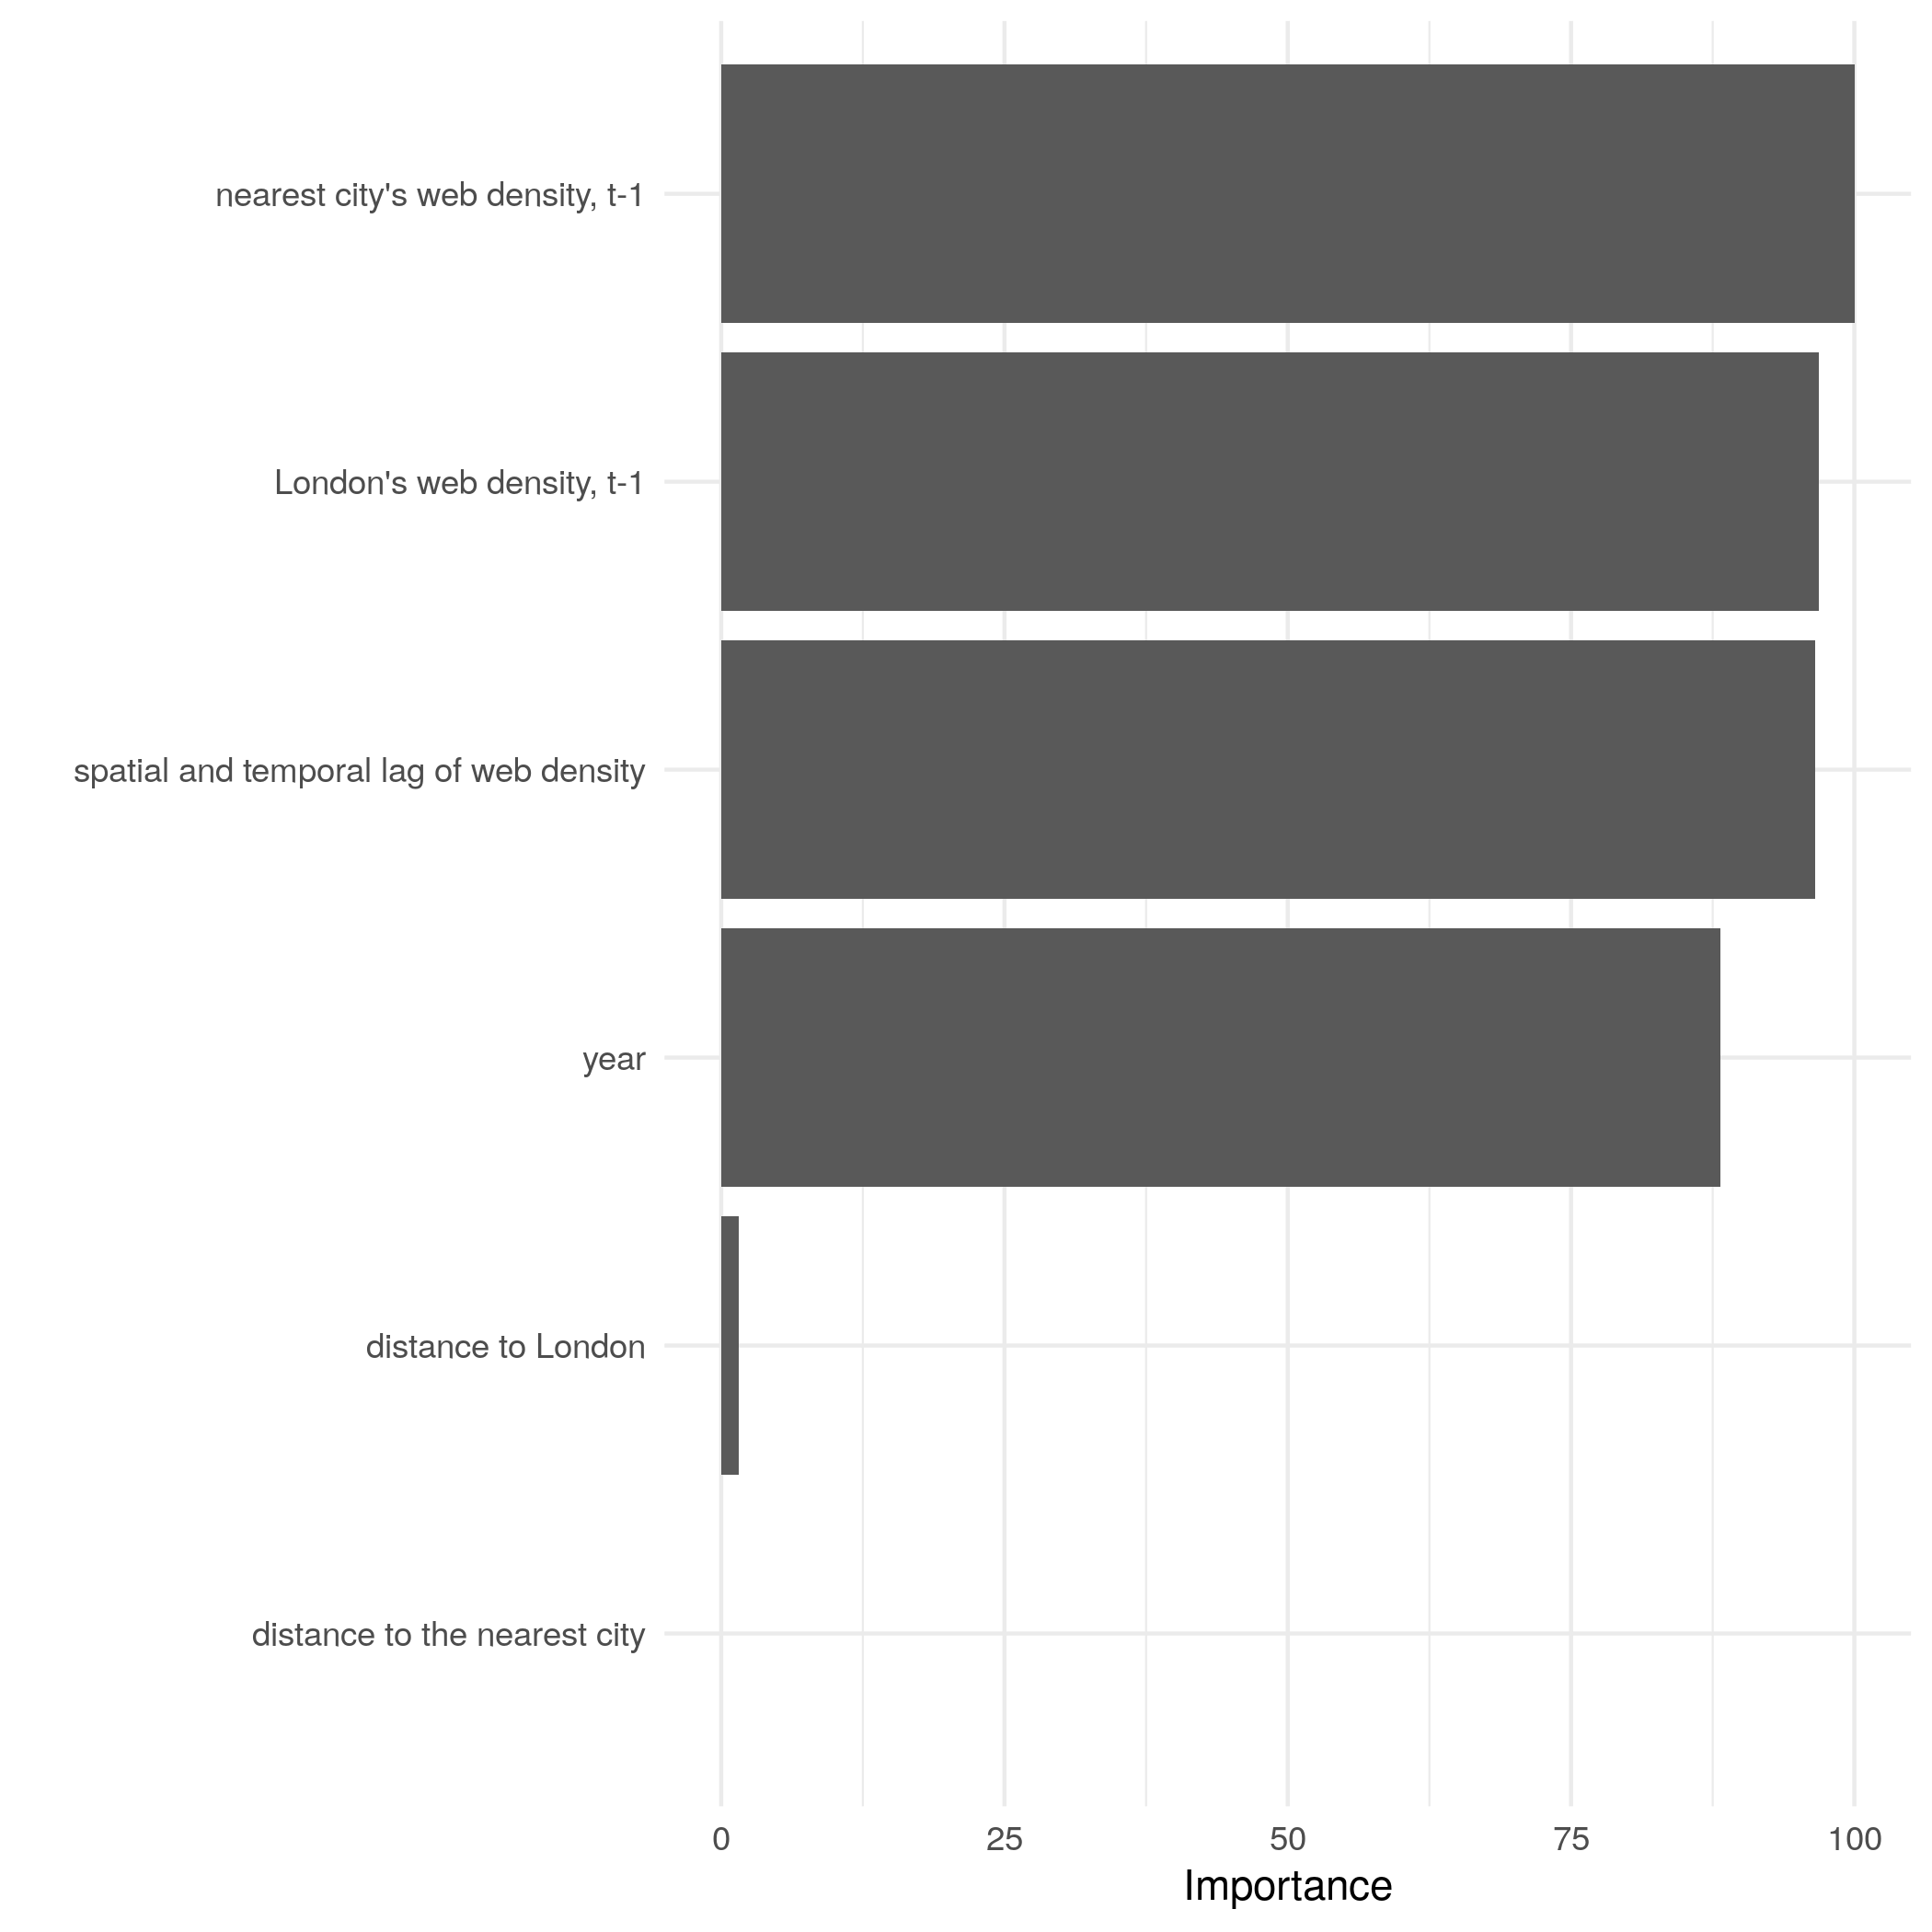
\includegraphics[width=1\textwidth,height=\textheight]{../../outputs/rf/figures/varimp_LA.png}

}

\caption{\label{var.imp.LAD}Variable importance, LAD}

\end{figure}%

\begin{figure}[H]

{\centering 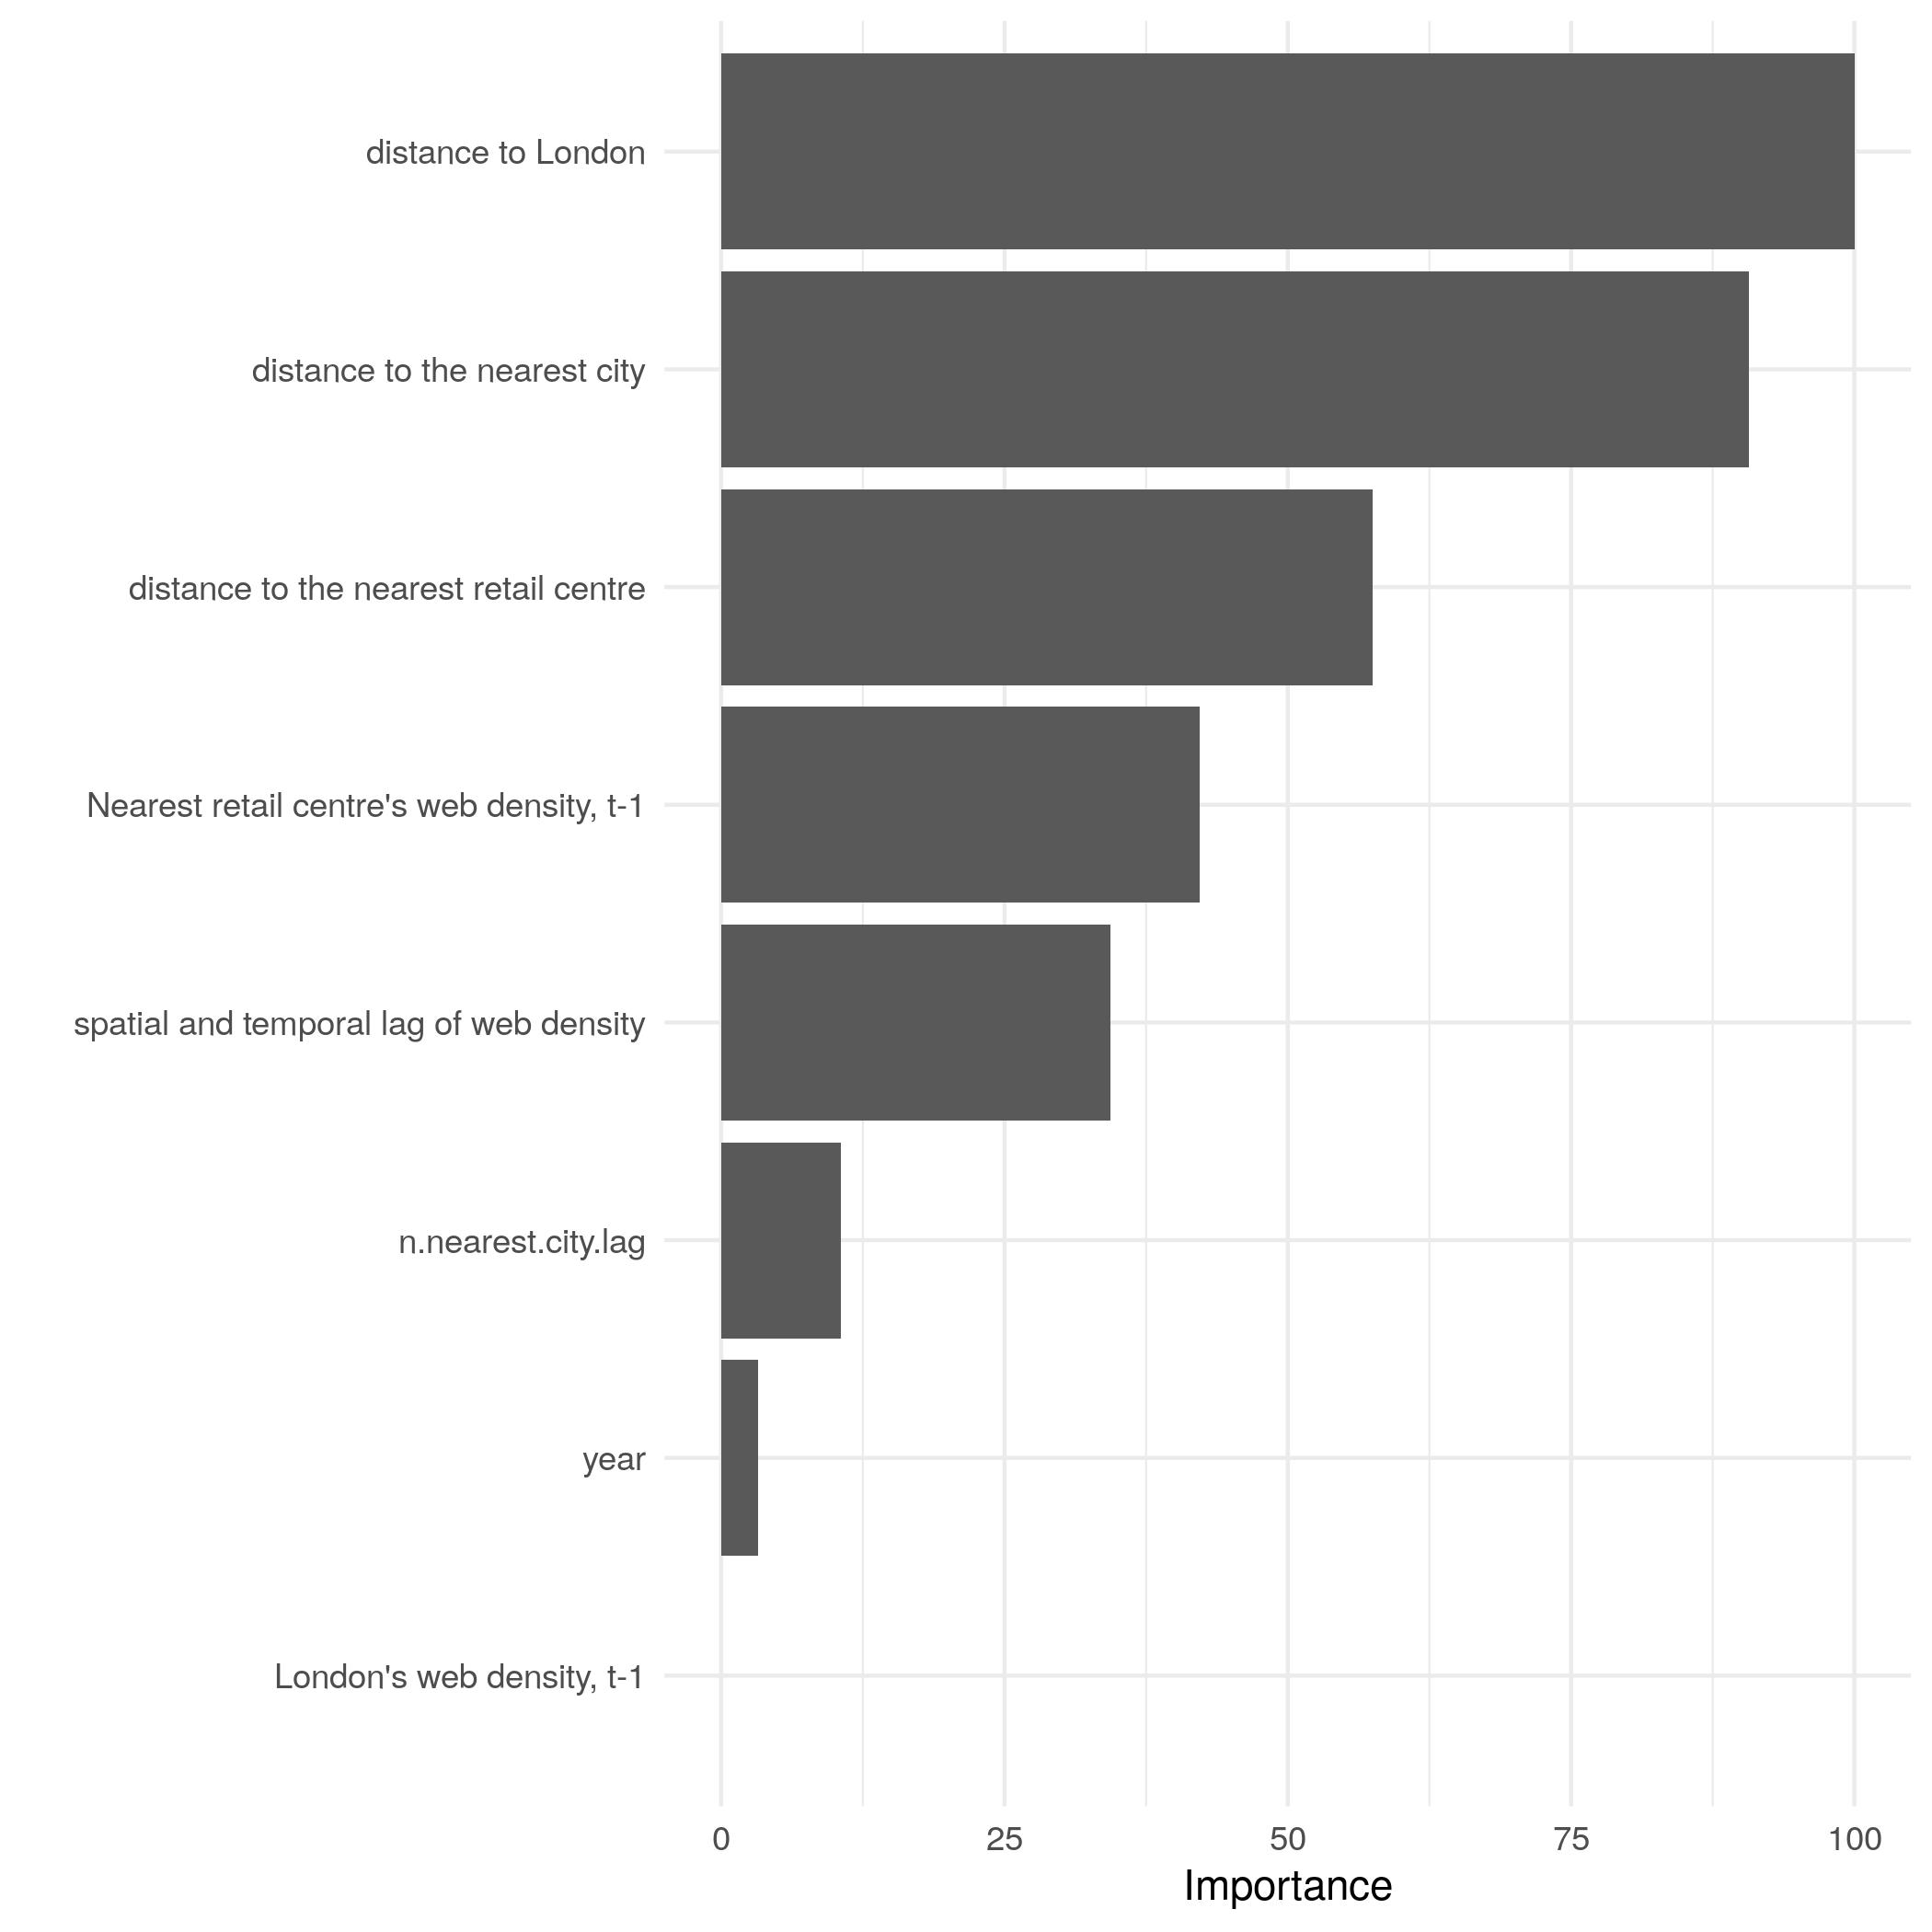
\includegraphics[width=1\textwidth,height=\textheight]{../../outputs/rf/figures/varimp_OA.png}

}

\caption{\label{var.imp.OA}Variable importance, OA}

\end{figure}%

Figure \ref{var.imp} to replace Figures \ref{var.imp.LAD} and
\ref{var.imp.OA} once I have the variable importance for LAD.

\begin{figure}[H]

{\centering 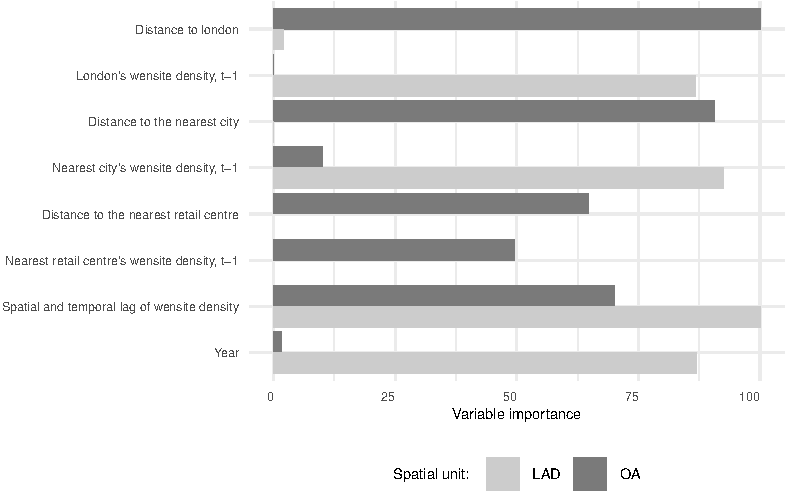
\includegraphics[width=1\textwidth,height=\textheight]{tranos2023_files/figure-pdf/varimp-1.pdf}

}

\caption{\label{var.imp}Variable importance}

\end{figure}%

Table \ref{table.regions} presents the results of the recursive hold out
models, which aim to highlight the potential regional heterogeneity of
the spatial processes behind the diffusion of web technologies. To begin
with, as highlighted before, there is a difference of magnitude of one
order between the LAD and the OA prediction errors, which is aligned
with previous results that employed all data points. What is of interest
here is the regional comparison. Table \ref{table.regions} illustrates
some striking similarities, but also a few significant differences. The
regions the web diffusion of which is better predicted using models
trained in the rest of the country are the same despite the scale of
analysis: South East, Wales, Yorkshire and The Humber and the North East
of England. In other words, these are the regions whose spatial
diffusion mechanisms of web technologies is closer to the country's
average. Despite the consistency across scales, this is a diverse set of
regions: \textbf{ADD CHARACTERISTICS}.

At the other end of the spectrum, Scotland's and the North West's web
diffusion mechanisms are consistently diverging from the country's
average. This should not come as a surprise as these regions are
characterised of high levels of rurality and remoteness. Similarly,
London diffusion mechanisms diverge from the country's average and this
is consistent across scales. London's uniqueness in UK's urban system
and economy is also reflected in the spatial diffusion mechanisms of web
technologies within its LAD and OA. It needs to be highlighted though
that the difference between the \(R^2\) of LAD and OA is more that an
order of magnitude signaling how difficult is to predict diffusion at
such a small spatial scale. Northern Ireland is an interesting case.
While it ranks at the bottom of the scale when the models are trained
and tested on LAD data, when the modelling adopts the more granular OA
scale, the spatial mechanisms that shape the web diffusion within this
region appear to be closer to the country's average. At this scale,
proximity, or lack of, relative to the rest of the country become less
important and the internal to the region spatial structure predictors
start playing a more important role \textbf{CHECK NI OA model}.

\begin{longtable}[]{@{}lrrrr@{}}
\caption{Regional differences\label{table.regions}}\tabularnewline
\toprule\noalign{}
Region & \(R^2\) LAD & Rank LAD & \(R^2\) OA & Rank OA \\
\midrule\noalign{}
\endfirsthead
\toprule\noalign{}
Region & \(R^2\) LAD & Rank LAD & \(R^2\) OA & Rank OA \\
\midrule\noalign{}
\endhead
\bottomrule\noalign{}
\endlastfoot
South East & 0.947 & 1 & 0.134 & 2 \\
Wales & 0.916 & 2 & 0.131 & 3 \\
Yorkshire and The Humber & 0.906 & 3 & 0.144 & 1 \\
North East & 0.895 & 4 & 0.128 & 4 \\
West Midlands & 0.883 & 5 & 0.070 & 9 \\
East Midlands & 0.882 & 6 & 0.088 & 8 \\
East of England & 0.876 & 7 & 0.106 & 6 \\
South West & 0.864 & 8 & 0.117 & 5 \\
London & 0.805 & 9 & 0.055 & 10 \\
Scotland & 0.770 & 10 & 0.035 & 11 \\
North West & 0.664 & 11 & 0.017 & 12 \\
Nortern Ireland & 0.576 & 12 & 0.101 & 7 \\
\end{longtable}

\section{Discussion and conclusions}\label{sec-conclusions}

contrary to results from future studies regarding social media
\citep{lengyel2020role}, web technologies did not exclusively spread
from a central location.

\setcounter{section}{0}
\renewcommand{\thesection}{\Alph{section}}

\setcounter{table}{0}
\renewcommand{\thetable}{A\arabic{table}}

\setcounter{figure}{0}
\renewcommand{\thefigure}{A\arabic{figure}}

\section{Appendices}\label{appendices}

\counterwithin{figure}{section}
\counterwithin{table}{section}

\subsection{\texorpdfstring{\(t_0\) estunates for all
LAD}{t\_0 estunates for all LAD}}\label{t_0-estunates-for-all-lad}

\begin{longtable}[]{@{}
  >{\raggedright\arraybackslash}p{(\columnwidth - 8\tabcolsep) * \real{0.4091}}
  >{\centering\arraybackslash}p{(\columnwidth - 8\tabcolsep) * \real{0.1818}}
  >{\centering\arraybackslash}p{(\columnwidth - 8\tabcolsep) * \real{0.1364}}
  >{\centering\arraybackslash}p{(\columnwidth - 8\tabcolsep) * \real{0.0795}}
  >{\centering\arraybackslash}p{(\columnwidth - 8\tabcolsep) * \real{0.1932}}@{}}
\caption{S-curve estiamtes for LAD\label{table.s.lads}}\tabularnewline
\toprule\noalign{}
\begin{minipage}[b]{\linewidth}\raggedright
LAD
\end{minipage} & \begin{minipage}[b]{\linewidth}\centering
\(t_0\) estimate
\end{minipage} & \begin{minipage}[b]{\linewidth}\centering
Std. error
\end{minipage} & \begin{minipage}[b]{\linewidth}\centering
\(R^2\)
\end{minipage} & \begin{minipage}[b]{\linewidth}\centering
Diffusion speed
\end{minipage} \\
\midrule\noalign{}
\endfirsthead
\toprule\noalign{}
\begin{minipage}[b]{\linewidth}\raggedright
LAD
\end{minipage} & \begin{minipage}[b]{\linewidth}\centering
\(t_0\) estimate
\end{minipage} & \begin{minipage}[b]{\linewidth}\centering
Std. error
\end{minipage} & \begin{minipage}[b]{\linewidth}\centering
\(R^2\)
\end{minipage} & \begin{minipage}[b]{\linewidth}\centering
Diffusion speed
\end{minipage} \\
\midrule\noalign{}
\endhead
\bottomrule\noalign{}
\endlastfoot
Horsham & 2001.423 & 0.254 & 0.950 & fast \\
Fareham & 2001.443 & 0.346 & 0.925 & fast \\
Kingston upon Thames & 2001.513 & 0.354 & 0.933 & fast \\
Kensington and Chelsea & 2001.581 & 0.341 & 0.943 & fast \\
Runnymede & 2001.582 & 0.266 & 0.943 & fast \\
Bracknell Forest & 2001.586 & 0.324 & 0.928 & fast \\
Elmbridge & 2001.656 & 0.333 & 0.932 & fast \\
Reigate and Banstead & 2001.665 & 0.253 & 0.964 & fast \\
South Cambridgeshire & 2001.680 & 0.433 & 0.905 & fast \\
Walsall & 2001.715 & 0.413 & 0.901 & fast \\
Surrey Heath & 2001.718 & 0.333 & 0.933 & fast \\
Woking & 2001.759 & 0.292 & 0.951 & fast \\
South Norfolk & 2001.874 & 0.358 & 0.931 & fast \\
City of London & 2001.874 & 0.499 & 0.930 & fast \\
Wokingham & 2001.891 & 0.287 & 0.958 & fast \\
Reading & 2001.900 & 0.318 & 0.948 & fast \\
Sevenoaks & 2001.904 & 0.407 & 0.926 & fast \\
Huntingdonshire & 2001.912 & 0.402 & 0.925 & fast \\
Pendle & 2001.924 & 0.407 & 0.923 & fast \\
St Albans & 2001.933 & 0.396 & 0.927 & fast \\
Perth and Kinross & 2001.943 & 0.228 & 0.970 & fast \\
Bromley & 2001.945 & 0.396 & 0.919 & fast \\
Rushmoor & 2001.962 & 0.518 & 0.912 & fast \\
Powys & 2001.969 & 0.278 & 0.963 & fast \\
Swindon & 2001.996 & 0.390 & 0.916 & fast \\
Chelmsford & 2002.008 & 0.545 & 0.911 & fast \\
Crawley & 2002.008 & 0.379 & 0.949 & fast \\
Dumfries and Galloway & 2002.012 & 0.251 & 0.967 & fast \\
Inverclyde & 2002.030 & 0.330 & 0.915 & fast \\
North Hertfordshire & 2002.031 & 0.475 & 0.920 & fast \\
Moray & 2002.050 & 0.358 & 0.947 & fast \\
Orkney Islands & 2002.070 & 0.283 & 0.958 & fast \\
Fife & 2002.070 & 0.363 & 0.945 & fast \\
Mole Valley & 2002.071 & 0.460 & 0.925 & fast \\
Guildford & 2002.113 & 0.413 & 0.941 & fast \\
Buckinghamshire & 2002.114 & 0.390 & 0.942 & fast \\
Cotswold & 2002.116 & 0.375 & 0.946 & fast \\
Shetland Islands & 2002.120 & 0.332 & 0.949 & fast \\
South Oxfordshire & 2002.146 & 0.367 & 0.950 & fast \\
Watford & 2002.157 & 0.451 & 0.929 & fast \\
Aberdeenshire & 2002.168 & 0.416 & 0.931 & fast \\
Southampton & 2002.189 & 0.472 & 0.922 & fast \\
Mid Suffolk & 2002.196 & 0.442 & 0.922 & fast \\
Eden & 2002.196 & 0.334 & 0.949 & fast \\
South Lakeland & 2002.197 & 0.238 & 0.974 & fast \\
Stoke-on-Trent & 2002.203 & 0.419 & 0.927 & fast \\
Babergh & 2002.209 & 0.449 & 0.927 & fast \\
Bexley & 2002.213 & 0.493 & 0.909 & fast \\
Torbay & 2002.215 & 0.374 & 0.942 & fast \\
Brentwood & 2002.219 & 0.336 & 0.936 & fast \\
Ceredigion & 2002.227 & 0.241 & 0.971 & fast \\
Spelthorne & 2002.232 & 0.451 & 0.933 & fast \\
Bath and North East Somerset & 2002.238 & 0.402 & 0.941 & fast \\
Falkirk & 2002.245 & 0.367 & 0.938 & fast \\
Broxtowe & 2002.258 & 0.435 & 0.932 & fast \\
East Hertfordshire & 2002.261 & 0.453 & 0.928 & fast \\
Stirling & 2002.268 & 0.251 & 0.975 & fast \\
Ealing & 2002.294 & 0.523 & 0.922 & fast \\
Mid Sussex & 2002.295 & 0.453 & 0.936 & fast \\
Barrow-in-Furness & 2002.303 & 0.284 & 0.959 & fast \\
West Oxfordshire & 2002.322 & 0.467 & 0.929 & fast \\
Sutton & 2002.326 & 0.544 & 0.911 & fast \\
Portsmouth & 2002.356 & 0.479 & 0.921 & fast \\
Great Yarmouth & 2002.369 & 0.265 & 0.968 & fast \\
East Hampshire & 2002.370 & 0.474 & 0.931 & fast \\
Wyre Forest & 2002.376 & 0.561 & 0.916 & fast \\
Angus & 2002.378 & 0.396 & 0.939 & fast \\
Argyll and Bute & 2002.427 & 0.321 & 0.962 & fast \\
Scottish Borders & 2002.428 & 0.298 & 0.962 & fast \\
East Suffolk & 2002.431 & 0.533 & 0.919 & fast \\
Blackpool & 2002.443 & 0.294 & 0.962 & fast \\
Cherwell & 2002.448 & 0.533 & 0.923 & fast \\
Wandsworth & 2002.449 & 0.570 & 0.921 & fast \\
Tendring & 2002.456 & 0.456 & 0.935 & fast \\
Westminster & 2002.459 & 0.437 & 0.952 & fast \\
Richmond upon Thames & 2002.462 & 0.389 & 0.956 & fast \\
Test Valley & 2002.463 & 0.553 & 0.920 & fast \\
Isle of Wight & 2002.478 & 0.377 & 0.953 & fast \\
Vale of White Horse & 2002.496 & 0.408 & 0.949 & fast \\
Croydon & 2002.510 & 0.504 & 0.927 & fast \\
Hounslow & 2002.521 & 0.426 & 0.952 & fast \\
Copeland & 2002.524 & 0.237 & 0.971 & fast \\
Wiltshire & 2002.528 & 0.450 & 0.940 & fast \\
Gwynedd & 2002.536 & 0.372 & 0.954 & fast \\
Hillingdon & 2002.560 & 0.470 & 0.940 & fast \\
Conwy & 2002.564 & 0.372 & 0.954 & fast \\
Highland & 2002.566 & 0.270 & 0.972 & fast \\
Basingstoke and Deane & 2002.572 & 0.461 & 0.947 & fast \\
Harrow & 2002.587 & 0.509 & 0.936 & fast \\
West Berkshire & 2002.595 & 0.696 & 0.902 & fast \\
North Lincolnshire & 2002.596 & 0.501 & 0.933 & fast \\
East Dunbartonshire & 2002.598 & 0.528 & 0.925 & fast \\
Bradford & 2002.598 & 0.613 & 0.916 & fast \\
Waverley & 2002.606 & 0.512 & 0.928 & fast \\
Stroud & 2002.608 & 0.559 & 0.916 & fast \\
Herefordshire, County of & 2002.622 & 0.388 & 0.956 & fast \\
North Norfolk & 2002.624 & 0.422 & 0.945 & fast \\
Nottingham & 2002.630 & 0.531 & 0.936 & fast \\
Castle Point & 2002.645 & 0.470 & 0.936 & fast \\
North Warwickshire & 2002.657 & 0.380 & 0.955 & fast \\
Gravesham & 2002.680 & 0.473 & 0.933 & fast \\
Lancaster & 2002.692 & 0.336 & 0.963 & fast \\
West Suffolk & 2002.699 & 0.536 & 0.930 & fast \\
Stafford & 2002.719 & 0.499 & 0.933 & fast \\
Tunbridge Wells & 2002.720 & 0.401 & 0.958 & fast \\
Oxford & 2002.723 & 0.583 & 0.934 & fast \\
East Lothian & 2002.731 & 0.537 & 0.927 & fast \\
Redcar and Cleveland & 2002.750 & 0.509 & 0.929 & fast \\
Tamworth & 2002.755 & 0.551 & 0.929 & fast \\
South Hams & 2002.773 & 0.422 & 0.952 & fast \\
Allerdale & 2002.784 & 0.376 & 0.958 & fast \\
Central Bedfordshire & 2002.825 & 0.620 & 0.921 & fast \\
East Cambridgeshire & 2002.843 & 0.636 & 0.927 & fast \\
Havant & 2002.853 & 0.541 & 0.932 & fast \\
South Lanarkshire & 2002.874 & 0.486 & 0.938 & fast \\
Stratford-on-Avon & 2002.879 & 0.470 & 0.945 & fast \\
Arun & 2002.882 & 0.526 & 0.938 & fast \\
Fenland & 2002.891 & 0.632 & 0.918 & fast \\
Monmouthshire & 2002.893 & 0.501 & 0.935 & fast \\
Denbighshire & 2002.901 & 0.457 & 0.947 & fast \\
Southend-on-Sea & 2002.903 & 0.551 & 0.932 & fast \\
High Peak & 2002.903 & 0.488 & 0.946 & fast \\
Pembrokeshire & 2002.905 & 0.387 & 0.958 & fast \\
Malvern Hills & 2002.907 & 0.524 & 0.940 & fast \\
Camden & 2002.915 & 0.599 & 0.941 & fast \\
North Devon & 2002.926 & 0.426 & 0.950 & fast \\
Wyre & 2002.927 & 0.553 & 0.927 & fast \\
Darlington & 2002.933 & 0.615 & 0.929 & fast \\
Swale & 2002.940 & 0.447 & 0.948 & fast \\
Welwyn Hatfield & 2002.951 & 0.628 & 0.922 & fast \\
Mid Devon & 2002.960 & 0.485 & 0.946 & fast \\
Lewes & 2002.964 & 0.507 & 0.945 & fast \\
Dorset & 2002.968 & 0.407 & 0.958 & fast \\
Brighton and Hove & 2002.976 & 0.578 & 0.934 & fast \\
Braintree & 2002.978 & 0.534 & 0.938 & fast \\
Epsom and Ewell & 2002.979 & 0.746 & 0.908 & fast \\
Sefton & 2002.980 & 0.616 & 0.928 & fast \\
Eastleigh & 2002.992 & 0.595 & 0.929 & fast \\
Craven & 2002.993 & 0.379 & 0.965 & fast \\
Hammersmith and Fulham & 2002.997 & 0.585 & 0.944 & fast \\
Greenwich & 2003.014 & 0.571 & 0.930 & slow \\
Cheltenham & 2003.025 & 0.602 & 0.937 & slow \\
Worcester & 2003.041 & 0.659 & 0.920 & slow \\
Tower Hamlets & 2003.043 & 0.660 & 0.926 & slow \\
New Forest & 2003.046 & 0.554 & 0.941 & slow \\
East Renfrewshire & 2003.046 & 0.739 & 0.900 & slow \\
Fylde & 2003.056 & 0.501 & 0.946 & slow \\
Carmarthenshire & 2003.067 & 0.390 & 0.958 & slow \\
West Lancashire & 2003.076 & 0.547 & 0.937 & slow \\
Hastings & 2003.086 & 0.685 & 0.911 & slow \\
Carlisle & 2003.111 & 0.541 & 0.934 & slow \\
Wychavon & 2003.115 & 0.570 & 0.935 & slow \\
Isle of Anglesey & 2003.144 & 0.403 & 0.960 & slow \\
Dudley & 2003.150 & 0.678 & 0.925 & slow \\
Ryedale & 2003.152 & 0.380 & 0.961 & slow \\
Rother & 2003.162 & 0.366 & 0.966 & slow \\
Leicester & 2003.167 & 0.686 & 0.924 & slow \\
Breckland & 2003.182 & 0.567 & 0.938 & slow \\
Tandridge & 2003.190 & 0.747 & 0.918 & slow \\
Shropshire & 2003.206 & 0.621 & 0.928 & slow \\
West Devon & 2003.228 & 0.489 & 0.949 & slow \\
Milton Keynes & 2003.231 & 0.700 & 0.929 & slow \\
Sandwell & 2003.234 & 0.760 & 0.916 & slow \\
Winchester & 2003.234 & 0.443 & 0.956 & slow \\
Redditch & 2003.238 & 0.706 & 0.923 & slow \\
Rugby & 2003.265 & 0.709 & 0.922 & slow \\
North Somerset & 2003.278 & 0.558 & 0.939 & slow \\
West Lindsey & 2003.285 & 0.674 & 0.924 & slow \\
Richmondshire & 2003.286 & 0.425 & 0.958 & slow \\
Melton & 2003.292 & 0.534 & 0.946 & slow \\
Chichester & 2003.295 & 0.582 & 0.942 & slow \\
Torridge & 2003.301 & 0.532 & 0.942 & slow \\
Dundee City & 2003.303 & 0.568 & 0.939 & slow \\
South Ayrshire & 2003.303 & 0.626 & 0.931 & slow \\
East Devon & 2003.308 & 0.492 & 0.947 & slow \\
Bolton & 2003.323 & 0.774 & 0.913 & slow \\
Hertsmere & 2003.326 & 0.726 & 0.924 & slow \\
Bournemouth, Christchurch and Poole & 2003.347 & 0.662 & 0.936 & slow \\
Maldon & 2003.349 & 0.495 & 0.951 & slow \\
Barnet & 2003.352 & 0.766 & 0.919 & slow \\
Brent & 2003.389 & 0.762 & 0.925 & slow \\
Midlothian & 2003.413 & 0.732 & 0.921 & slow \\
Boston & 2003.416 & 0.593 & 0.933 & slow \\
Scarborough & 2003.421 & 0.431 & 0.963 & slow \\
Kirklees & 2003.435 & 0.725 & 0.925 & slow \\
Tameside & 2003.441 & 0.819 & 0.907 & slow \\
Newport & 2003.449 & 0.635 & 0.930 & slow \\
Glasgow City & 2003.451 & 0.759 & 0.922 & slow \\
Clackmannanshire & 2003.454 & 0.585 & 0.936 & slow \\
Three Rivers & 2003.458 & 0.628 & 0.947 & slow \\
Harborough & 2003.488 & 0.549 & 0.950 & slow \\
Rochdale & 2003.496 & 0.685 & 0.937 & slow \\
Tonbridge and Malling & 2003.497 & 0.710 & 0.927 & slow \\
Somerset West and Taunton & 2003.502 & 0.491 & 0.955 & slow \\
Wrexham & 2003.512 & 0.553 & 0.942 & slow \\
Worthing & 2003.522 & 0.622 & 0.938 & slow \\
Tewkesbury & 2003.540 & 0.580 & 0.946 & slow \\
City of Edinburgh & 2003.541 & 0.685 & 0.941 & slow \\
Coventry & 2003.592 & 0.564 & 0.948 & slow \\
Northumberland & 2003.607 & 0.508 & 0.954 & slow \\
Mid and East Antrim & 2003.609 & 0.893 & 0.900 & slow \\
Wigan & 2003.617 & 0.755 & 0.929 & slow \\
Lichfield & 2003.629 & 0.625 & 0.939 & slow \\
Ashford & 2003.633 & 0.535 & 0.944 & slow \\
Cornwall & 2003.638 & 0.443 & 0.963 & slow \\
Mendip & 2003.652 & 0.505 & 0.955 & slow \\
Stevenage & 2003.665 & 0.525 & 0.958 & slow \\
Blaenau Gwent & 2003.666 & 0.643 & 0.933 & slow \\
Lincoln & 2003.666 & 0.634 & 0.940 & slow \\
South Somerset & 2003.676 & 0.553 & 0.948 & slow \\
Charnwood & 2003.677 & 0.699 & 0.934 & slow \\
North Ayrshire & 2003.682 & 0.607 & 0.942 & slow \\
Folkestone and Hythe & 2003.684 & 0.792 & 0.905 & slow \\
Eastbourne & 2003.684 & 0.697 & 0.930 & slow \\
Blackburn with Darwen & 2003.685 & 0.680 & 0.938 & slow \\
Dover & 2003.699 & 0.574 & 0.948 & slow \\
Adur & 2003.735 & 0.551 & 0.954 & slow \\
Haringey & 2003.739 & 0.667 & 0.943 & slow \\
Gosport & 2003.751 & 0.600 & 0.934 & slow \\
Trafford & 2003.752 & 0.640 & 0.949 & slow \\
Norwich & 2003.756 & 0.742 & 0.939 & slow \\
West Lothian & 2003.758 & 0.652 & 0.943 & slow \\
North East Lincolnshire & 2003.811 & 0.858 & 0.920 & slow \\
Bristol, City of & 2003.828 & 0.831 & 0.928 & slow \\
Rushcliffe & 2003.839 & 0.591 & 0.954 & slow \\
Hinckley and Bosworth & 2003.857 & 0.749 & 0.934 & slow \\
Torfaen & 2003.861 & 0.841 & 0.922 & slow \\
Swansea & 2003.875 & 0.650 & 0.947 & slow \\
Wolverhampton & 2003.882 & 0.793 & 0.931 & slow \\
Kingston upon Hull, City of & 2003.885 & 0.757 & 0.936 & slow \\
Calderdale & 2003.889 & 0.714 & 0.939 & slow \\
North Northamptonshire & 2003.902 & 0.746 & 0.935 & slow \\
Stockton-on-Tees & 2003.902 & 0.955 & 0.916 & slow \\
Wealden & 2003.906 & 0.736 & 0.938 & slow \\
Thanet & 2003.953 & 0.667 & 0.947 & slow \\
Broadland & 2003.962 & 0.727 & 0.938 & slow \\
West Northamptonshire & 2003.972 & 0.736 & 0.940 & slow \\
North Kesteven & 2003.976 & 0.633 & 0.942 & slow \\
Neath Port Talbot & 2003.981 & 0.767 & 0.933 & slow \\
Rhondda Cynon Taf & 2003.991 & 0.769 & 0.925 & slow \\
Enfield & 2003.992 & 0.588 & 0.954 & slow \\
East Lindsey & 2004.010 & 0.577 & 0.952 & slow \\
Teignbridge & 2004.015 & 0.681 & 0.941 & slow \\
York & 2004.025 & 0.739 & 0.944 & slow \\
Harlow & 2004.030 & 0.803 & 0.936 & slow \\
Vale of Glamorgan & 2004.033 & 0.592 & 0.951 & slow \\
Newark and Sherwood & 2004.034 & 0.668 & 0.946 & slow \\
Merton & 2004.041 & 0.932 & 0.922 & slow \\
Hambleton & 2004.065 & 0.636 & 0.953 & slow \\
Bedford & 2004.068 & 0.852 & 0.933 & slow \\
Stockport & 2004.075 & 0.757 & 0.942 & slow \\
South Ribble & 2004.126 & 0.674 & 0.948 & slow \\
Uttlesford & 2004.144 & 0.905 & 0.926 & slow \\
Rossendale & 2004.160 & 0.976 & 0.923 & slow \\
Oldham & 2004.162 & 0.801 & 0.938 & slow \\
Sheffield & 2004.189 & 0.770 & 0.944 & slow \\
Ribble Valley & 2004.204 & 0.718 & 0.945 & slow \\
Maidstone & 2004.222 & 0.854 & 0.932 & slow \\
Cheshire West and Chester & 2004.234 & 0.742 & 0.947 & slow \\
Thurrock & 2004.241 & 0.841 & 0.924 & slow \\
Telford and Wrekin & 2004.241 & 1.024 & 0.917 & slow \\
Cardiff & 2004.246 & 0.823 & 0.937 & slow \\
County Durham & 2004.250 & 0.626 & 0.953 & slow \\
Plymouth & 2004.252 & 0.785 & 0.934 & slow \\
Bridgend & 2004.256 & 0.547 & 0.956 & slow \\
Rotherham & 2004.273 & 0.722 & 0.938 & slow \\
Hyndburn & 2004.298 & 0.881 & 0.932 & slow \\
Newcastle upon Tyne & 2004.305 & 0.906 & 0.932 & slow \\
Wakefield & 2004.314 & 0.905 & 0.923 & slow \\
Havering & 2004.345 & 0.822 & 0.938 & slow \\
South Kesteven & 2004.353 & 1.026 & 0.915 & slow \\
Canterbury & 2004.354 & 0.602 & 0.960 & slow \\
Broxbourne & 2004.363 & 0.817 & 0.944 & slow \\
Peterborough & 2004.382 & 0.937 & 0.932 & slow \\
Redbridge & 2004.411 & 1.028 & 0.925 & slow \\
Bury & 2004.431 & 0.735 & 0.953 & slow \\
Harrogate & 2004.433 & 0.971 & 0.927 & slow \\
Birmingham & 2004.435 & 1.182 & 0.912 & slow \\
South Tyneside & 2004.446 & 0.636 & 0.948 & slow \\
Chorley & 2004.462 & 1.093 & 0.913 & slow \\
North East Derbyshire & 2004.483 & 0.703 & 0.953 & slow \\
Lambeth & 2004.485 & 0.958 & 0.937 & slow \\
Doncaster & 2004.496 & 0.672 & 0.953 & slow \\
South Gloucestershire & 2004.499 & 0.881 & 0.937 & slow \\
Caerphilly & 2004.499 & 0.819 & 0.938 & slow \\
East Staffordshire & 2004.501 & 1.132 & 0.910 & slow \\
North Tyneside & 2004.509 & 0.864 & 0.933 & slow \\
South Holland & 2004.534 & 0.851 & 0.941 & slow \\
Gateshead & 2004.535 & 0.869 & 0.934 & slow \\
St.~Helens & 2004.542 & 1.097 & 0.923 & slow \\
Flintshire & 2004.549 & 0.764 & 0.951 & slow \\
Selby & 2004.549 & 0.716 & 0.947 & slow \\
Belfast & 2004.556 & 1.332 & 0.906 & slow \\
Sedgemoor & 2004.613 & 0.540 & 0.966 & slow \\
Exeter & 2004.617 & 0.964 & 0.936 & slow \\
South Derbyshire & 2004.629 & 0.934 & 0.938 & slow \\
Derbyshire Dales & 2004.668 & 0.648 & 0.963 & slow \\
East Riding of Yorkshire & 2004.683 & 0.728 & 0.955 & slow \\
Basildon & 2004.691 & 1.067 & 0.925 & slow \\
Barking and Dagenham & 2004.800 & 1.198 & 0.916 & slow \\
Causeway Coast and Glens & 2004.834 & 1.024 & 0.928 & slow \\
North Lanarkshire & 2004.839 & 0.878 & 0.945 & slow \\
Chesterfield & 2004.887 & 1.173 & 0.927 & slow \\
Newcastle-under-Lyme & 2004.933 & 1.172 & 0.925 & slow \\
East Ayrshire & 2004.934 & 1.280 & 0.903 & slow \\
Nuneaton and Bedworth & 2004.956 & 0.950 & 0.941 & slow \\
Blaby & 2004.959 & 1.059 & 0.929 & slow \\
Leeds & 2004.979 & 0.836 & 0.956 & slow \\
Erewash & 2004.987 & 0.939 & 0.944 & slow \\
Bassetlaw & 2004.998 & 0.982 & 0.944 & slow \\
Hackney & 2005.026 & 1.157 & 0.934 & slow \\
Barnsley & 2005.055 & 0.912 & 0.942 & slow \\
Amber Valley & 2005.105 & 1.017 & 0.941 & slow \\
Colchester & 2005.144 & 1.250 & 0.927 & slow \\
Ashfield & 2005.176 & 1.073 & 0.942 & slow \\
Wirral & 2005.184 & 1.084 & 0.939 & slow \\
Knowsley & 2005.186 & 1.160 & 0.923 & slow \\
Windsor and Maidenhead & 2005.195 & 1.746 & 0.902 & slow \\
Bromsgrove & 2005.494 & 1.144 & 0.941 & slow \\
Liverpool & 2005.526 & 1.276 & 0.936 & slow \\
Staffordshire Moorlands & 2005.583 & 1.426 & 0.924 & slow \\
Islington & 2005.970 & 1.223 & 0.955 & slow \\
Warrington & 2006.015 & 1.387 & 0.942 & slow \\
Newham & 2006.078 & 1.908 & 0.907 & slow \\
Bolsover & 2006.188 & 1.143 & 0.957 & slow \\
Lisburn and Castlereagh & 2006.193 & 1.970 & 0.903 & slow \\
Manchester & 2006.449 & 1.434 & 0.950 & slow \\
Sunderland & 2006.479 & 1.679 & 0.928 & slow \\
South Staffordshire & 2006.490 & 1.837 & 0.922 & slow \\
Rutland & 2006.529 & 0.986 & 0.967 & slow \\
Cannock Chase & 2006.700 & 2.231 & 0.917 & slow \\
Mansfield & 2006.889 & 1.579 & 0.946 & slow \\
Ards and North Down & 2006.947 & 2.485 & 0.907 & slow \\
Halton & 2007.069 & 0.932 & 0.967 & slow \\
Burnley & 2007.372 & 2.286 & 0.919 & slow \\
Middlesbrough & 2010.074 & 5.297 & 0.900 & slow \\
Isles of Scilly & 2012.163 & 4.257 & 0.953 & slow \\
\end{longtable}


\renewcommand\refname{References}
  \bibliography{bibliography}


\end{document}
